\documentclass[14pt,a4paper]{extreport}

% Язык и шрифты (XeLaTeX, стандарт БГУ / ВАК РБ)
\usepackage{fontspec}
\usepackage[english,russian]{babel}
\setmainfont{Times New Roman}
\setsansfont{Arial}
\setmonofont[Scale=0.82]{Menlo}

% Тонкая типографика и защита от выхода строк за правое поле
\usepackage{microtype}
\hyphenpenalty=250
\exhyphenpenalty=50
\tolerance=2500
\emergencystretch=3.5em
\pretolerance=150
\righthyphenmin=2
\lefthyphenmin=2
\widowpenalty=10000
\clubpenalty=10000
\renewcommand{\topfraction}{0.85}
\renewcommand{\bottomfraction}{0.75}
\renewcommand{\textfraction}{0.12}
\renewcommand{\floatpagefraction}{0.75}

\hyphenation{
    кон-век-ци-он-но
    диф-фу-зи-он-ных
    три-ан-гу-ля-ци-ях
    сер-ти-фи-ка-ции
    мор-фо-мет-рии
    су-пер-пик-се-лей
    дис-кре-ти-за-ции
}

% Поля страницы по требованиям ОИТ и Инструкции ВАК РБ
\usepackage[
    left=30mm,
    top=20mm,
    right=15mm,
    bottom=20mm
]{geometry}
\usepackage{indentfirst}
\usepackage{setspace}
\usepackage{lastpage}

\setlength{\parindent}{1.25cm}
\renewcommand{\baselinestretch}{1.15}

% Цвета и гиперссылки
\usepackage{xcolor}
\definecolor{bsuBlue}{HTML}{1B365D}
\definecolor{bsuAccent}{HTML}{27568B}
\definecolor{bsuSoft}{HTML}{F0F4F9}
\definecolor{bsuGreen}{HTML}{1E6B43}
\definecolor{bsuSoftGreen}{HTML}{EBF7F0}
\definecolor{bsuAmber}{HTML}{9C5700}
\definecolor{bsuSoftAmber}{HTML}{FEF6E9}

\usepackage[unicode]{hyperref}
\hypersetup{
    pdfstartview=FitH,
    colorlinks=true,
    linkcolor=black,
    urlcolor=bsuAccent,
    citecolor=black,
    bookmarksnumbered=true,
    unicode=true,
    pdftitle={Межмасштабный перенос графовых моделей и сертификация морфометрии изображений},
    pdfauthor={Довгий Александр Сергеевич}
}

% Математика
\usepackage{amsmath,amsfonts,amssymb,amsthm,mathtools,bm}

% Графика, векторные схемы TikZ и адаптивные таблицы строго в ширину листа
\usepackage{graphicx}
\usepackage{booktabs}
\usepackage{tabularx}
\usepackage{array}
\usepackage{makecell}
\usepackage{multirow}
\usepackage{float}
\usepackage{tikz}
\usetikzlibrary{arrows.meta,positioning,shapes.geometric,calc,fit,backgrounds}

% Типы колонок tabularx с переносом без переполнения
\newcolumntype{Y}{>{\raggedright\arraybackslash}X}
\newcolumntype{C}{>{\centering\arraybackslash}X}
\newcolumntype{R}{>{\raggedleft\arraybackslash}X}

% Подписи к рисункам и таблицам по стандарту ВАК РБ (тире, без точки в конце)
\usepackage[singlelinecheck=false]{caption}
\DeclareCaptionLabelSeparator{emdash}{ -- }
\captionsetup{labelsep=emdash}
\captionsetup[figure]{justification=centering, font={small, bf}, skip=6pt}
\captionsetup[table]{justification=raggedright, singlelinecheck=false, font={small, bf}, indention=0pt, skip=5pt}
\addto\captionsrussian{\renewcommand{\figurename}{Рисунок}}

% Оформление глав и разделов (аналогично магистерской диссертации)
\usepackage{titlesec}

\makeatletter
\renewcommand*\l@chapter[2]{%
  \ifnum \c@tocdepth >\m@ne
    \addpenalty{-\@highpenalty}%
    \vskip 0.8em \@plus\p@
    \setlength\@tempdima{1.5em}%
    \begingroup
      \parindent \z@ \rightskip \@pnumwidth
      \parfillskip -\@pnumwidth
      \leavevmode \bfseries
      \advance\leftskip\@tempdima
      \hskip -\leftskip
      #1\nobreak\normalfont\leaders\hbox{$\m@th
        \mkern \@dotsep mu\hbox{.}\mkern \@dotsep
        mu$}\hfill\nobreak\hb@xt@\@pnumwidth{\hss #2}\par
      \penalty\@highpenalty
    \endgroup
  \fi}
\makeatother

\titleformat{\chapter}[display]
{\centering\large\bfseries}{\chaptertitlename\ \thechapter}{8pt}{\large}
\titlespacing*{\chapter}{0pt}{-18pt}{20pt}

\titleformat{\section}[block]
  {\normalsize\bfseries}
  {\thesection\ }{0pt}{}
\titlespacing{\section}
  {\parindent}{2.6ex plus 0.8ex minus .2ex}{1.6ex plus .2ex}

\titleformat{\subsection}[block]
  {\normalsize\bfseries}
  {\thesubsection\ }{0pt}{}
\titlespacing{\subsection}
  {\parindent}{2.2ex plus 0.6ex minus .2ex}{1.2ex plus .2ex}

\addto\captionsrussian{%
  \renewcommand{\contentsname}{\centering\large ОГЛАВЛЕНИЕ}%
  \renewcommand{\chaptername}{ГЛАВА}
  \renewcommand{\chaptertitlename}{ГЛАВА}
}

% Компактные списки и нумерация литературы ВАК
\usepackage{enumitem}
\setlist{nosep, labelindent=\parindent, leftmargin=*, labelsep=0.5em}

\newcounter{litcnt}
\newcommand{\lititem}[1]{%
  \par\vspace{0.25ex}\refstepcounter{litcnt}\label{#1}%
  \noindent\hspace{0pt}\makebox[2.0em][l]{\thelitcnt.}\hangindent=2.0em\hangafter=1\ignorespaces
}

\newcounter{alitcnt}
\renewcommand{\thealitcnt}{\arabic{alitcnt}-А}
\newcommand{\alititem}[1]{%
  \par\vspace{0.25ex}\refstepcounter{alitcnt}\label{#1}%
  \noindent\hspace{0pt}\makebox[2.8em][l]{\thealitcnt.}\hangindent=2.8em\hangafter=1\ignorespaces
}

\DeclareMathOperator{\divop}{div}
\DeclareMathOperator{\diam}{diam}
\DeclareMathOperator{\diag}{diag}
\DeclareMathOperator{\Pe}{Pe}

\newcommand{\Real}{\mathbb{R}}
\newcommand{\calT}{\mathcal{T}}
\newcommand{\calN}{\mathcal{N}}
\newcommand{\calM}{\mathcal{M}}
\newcommand{\calL}{\mathcal{L}}
\newcommand{\calP}{\mathcal{P}}

\begin{document}

% !TeX root = ./main.tex

\setcounter{page}{1}
\thispagestyle{empty}
\setstretch{1.05}

\begin{center}
    {\bfseries БЕЛОРУССКИЙ ГОСУДАРСТВЕННЫЙ УНИВЕРСИТЕТ}\\[0.35cm]
    {\small Факультет прикладной математики и информатики}\\
    {\small Кафедра теории вероятностей и математической статистики}
\end{center}

\vspace{0.8cm}

\noindent УДК 004.852, 004.932, 519.63

\vspace{1.2cm}

\begin{center}
    {\Large\bfseries Довгий Александр Сергеевич}
\end{center}

\vspace{0.7cm}

\begin{center}
    {\large\bfseries МЕЖМАСШТАБНЫЙ ПЕРЕНОС ГРАФОВЫХ МОДЕЛЕЙ И СЕРТИФИКАЦИЯ МОРФОМЕТРИИ ИЗОБРАЖЕНИЙ}\\[0.9cm]
    {\normalsize Реферат по дисциплине}\\
    {\normalsize\bfseries «Основы информационных технологий»}
\end{center}

\vspace{1.4cm}

\begin{flushright}
\begin{minipage}{0.62\textwidth}
    \small\setstretch{1.15}
    Магистранта кафедры теории вероятностей\\
    и математической статистики ФПМИ БГУ\\[0.2cm]
    Специальность: 7-06-0533-05~-- Прикладная\\
    математика и информатика\\
    (профилизация «Компьютерный анализ данных»)\\[0.2cm]
    Научный руководитель:\\
    д-р техн. наук, доцент А.~М.~Недзьведь\\[0.2cm]
    E-mail: \texttt{aliaksandr\_douhi@epam.com}\\[0.45cm]
    Рецензент:\\[0.35cm]
    \rule{\textwidth}{0.4pt}
\end{minipage}
\end{flushright}

\vfill

\begin{center}
    Минск, 2026
\end{center}

\clearpage


\tableofcontents
\newpage

% !TeX root = ./main.tex

\chapter*{\large ВВЕДЕНИЕ}
\addcontentsline{toc}{chapter}{ВВЕДЕНИЕ}

Современный этап цифровой трансформации науки, биомедицинской диагностики и инженерного компьютерного моделирования характеризуется переходом от изолированных эмпирических алгоритмов обработки растровых сигналов к физически согласованным информационным технологиям анализа пространственно-временных данных~[\ref{itm:samarsky}, с.~14;~\ref{itm:kharin}, с.~22]. В задачах количественной микроскопии живых клеток, цифровой гистопатологии и экологического мониторинга регистрируемые кадры представляют собой дискретные выборки непрерывного физического поля (интенсивности флуоресценции, концентрации маркера или оптической плотности), эволюционирующего на ограниченной двумерной области.

Ключевая научно-технологическая проблема состоит в том, что пространственное разрешение и топология графа наблюдений существенно различаются между этапом обучения модели и этапом её лабораторной или клинической эксплуатации. При регистрации длительных обучающих серий в цейтраферной флуоресцентной микроскопии операторы применяют аппаратный биннинг пикселей матрицы (усреднение блоков $4\times 4$ или $6\times 6$) для снижения фототоксичности лазерного облучения, подавления фотовыцветания флуорофора и ускорения кадровой развёртки~[\ref{itm:nedzvedz2012}, с.~52]. На этапе же прецизионной морфометрической диагностики обученная модель применяется к кадрам полного разрешения (с ростом числа узлов в $8\text{--}10$~раз), нерегулярным адаптивным триангуляциям Делоне либо графам смежности суперпикселей~[\ref{itm:skimage}].

Классические графовые нейронные сети (ГНС), построенные на комбинаторной передаче сообщений по списку смежности~[\ref{itm:gasnikov}, с.~68;~\ref{itm:grand}], в подобных условиях теряют работоспособность: при измельчении шага сетки $h_G$ разности признаков сжимаются, рёберное внимание искажает масштаб времени, а локальные вентили переключателей вырождаются без переобучения весов~[\ref{itm:a1},~\ref{itm:a3}]. Высокая мировая актуальность проблемы подтверждается более чем $35$-кратным ростом числа научных работ по инвариантным к дискретизации нейронным операторам и графовым уравнениям в частных производных (УЧП) в архиве \texttt{arXiv.org}~[\ref{itm:arxiv}] и в базе \texttt{ScienceDirect}~[\ref{itm:sciencedirect}] за 2018--2026~гг. (рисунок~\ref{fig:pub_dynamics}).

\begin{figure}[htbp]
    \centering
    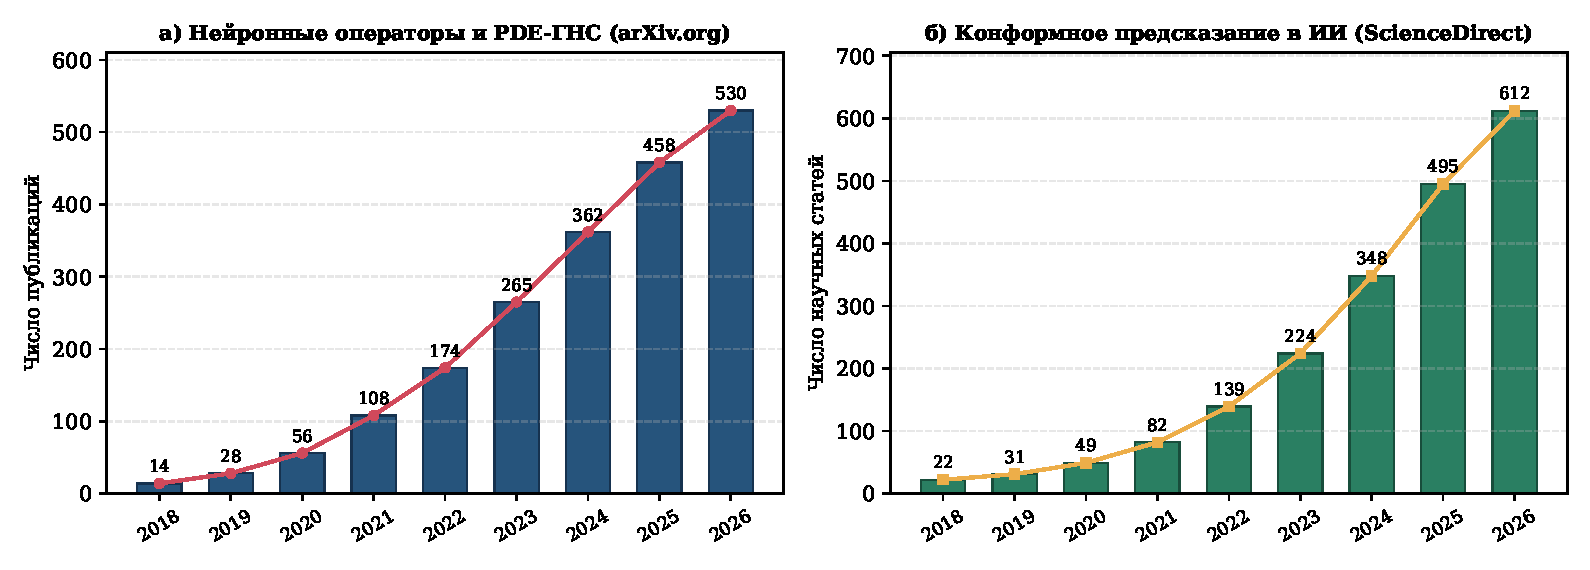
\includegraphics[width=0.98\textwidth]{figures/fig1_pub_dynamics.pdf}
    \caption{Динамика числа научных публикаций за 2018--2026~гг.: а)~по нейронным операторам и графовым УЧП в базе \texttt{arXiv.org}; б)~по конформному предсказанию в ИИ и анализе изображений в базе \texttt{ScienceDirect}}
    \label{fig:pub_dynamics}
\end{figure}

Анализ степени разработанности темы показывает, что спектральные теории переносимости ГНС~[\ref{itm:levie}] опираются на самосопряжённость оператора Лапласа и неприменимы к направленному конвективному сносу, а предельные модели на плотных графонах~[\ref{itm:medvedev},~\ref{itm:yan}] порождают экспоненциально растущие по времени оценки погрешности $\exp(CT)$ и не описывают разреженные планарные сетки. В свою очередь, эмпирические нейронные операторы~[\ref{itm:calvello},~\ref{itm:gfunk}] не снабжают прогнозируемые морфометрические показатели статистически достоверными границами ошибки без запуска эталонного решателя высокого разрешения. Тем самым в современной инженерии научных информационных систем сформировался разрыв между высокой скоростью обучения графовых суррогатов на грубых данных и требованиями метрологической надёжности при их переносе на целевые сетки диагностики.

Целью реферата является систематизация современных информационных технологий моделирования процессов переноса на графах и разработка программно-алгоритмического комплекса \texttt{CDQuad}, обеспечивающего перенос без дообучения адаптивных конвекционно-диффузионных моделей между сетками разного разрешения со статистической сертификацией ошибки морфометрических измерений на открытом стеке языка Python (\texttt{NumPy}, \texttt{SciPy}~[\ref{itm:scipy}], \texttt{scikit-image}~[\ref{itm:skimage}]).

Методологическую основу и методы исследования составляют системный и сравнительный анализ научно-технической литературы и программных платформ, методы вариационного исчисления, кусочно-линейных конечных элементов и барицентрических конечных объёмов на триангуляциях Делоне, алгоритмы разреженной вычислительной линейной алгебры в форматах \texttt{CSR/CSC}, аппарат непараметрического раздельного конформного предсказания (\emph{split conformal prediction})~[\ref{itm:vovk},~\ref{itm:angelopoulos}] и воспроизводимый вычислительный эксперимент на синтетических и реальных биомедицинских изображениях.

\newpage

\chapter*{\large ОБЩАЯ ХАРАКТЕРИСТИКА РАБОТЫ}
\addcontentsline{toc}{chapter}{ОБЩАЯ ХАРАКТЕРИСТИКА РАБОТЫ}

\textbf{Ключевые слова:} ИНФОРМАЦИОННЫЕ ТЕХНОЛОГИИ АНАЛИЗА ДАННЫХ НА ГРАФАХ, ГРАФОВЫЕ ДИФФЕРЕНЦИАЛЬНЫЕ УРАВНЕНИЯ, КОНВЕКЦИЯ-ДИФФУЗИЯ, ПЕРЕНОСИМОСТЬ МЕЖДУ РАЗРЕШЕНИЯМИ, НЕЙРОННЫЕ ОПЕРАТОРЫ, ЧИСЛО ПЕКЛЕ, ДВОЙСТВЕННЫЙ СЛОВАРНЫЙ ДЕФЕКТ, КОНФОРМНОЕ ПРЕДСКАЗАНИЕ, МОРФОМЕТРИЯ ИЗОБРАЖЕНИЙ, ОТКРЫТОЕ ПРОГРАММНОЕ ОБЕСПЕЧЕНИЕ.

\textbf{Связь работы с научными программами (проектами), темами.} Тема реферата и магистерской диссертации соответствует приоритетному направлению «1.~Цифровые технологии и искусственный интеллект» Указа Президента Республики Беларусь от 1~апреля 2025~г. №~135 «О приоритетных направлениях научной, научно-технической и инновационной деятельности на 2026--2030~годы»~[\ref{itm:ukaz135}], положениям Государственной программы «Цифровое развитие Беларуси»~[\ref{itm:gosprog}] в части создания импортонезависимых алгоритмических и программных средств анализа данных и биомедицинских изображений, а также выполняется в рамках темы НИР кафедры теории вероятностей и математической статистики ФПМИ БГУ «Математические и компьютерные методы анализа данных на графах» (распоряжение по ФПМИ БГУ от 11.09.2026 №~47).

\textbf{Цель и задачи исследования.} Цель работы~-- обоснование, алгоритмизация и программная реализация континуально-согласованного класса адаптивных конвекционно-диффузионных графовых операторов \texttt{CDQuad} и процедуры статистической сертификации ошибки переноса для устойчивой морфометрии динамических структур на изображениях переменного разрешения. Задачи исследования:
\begin{enumerate}
    \item выполнить аналитический обзор литературы 2020--2026~гг. и сравнительный аудит программных библиотек научного машинного обучения на графах;
    \item установить асимптотический механизм вырождения комбинаторных конвекционно-диффузионных ГНС при измельчении шага сетки;
    \item разработать модульный программный комплекс \texttt{CDQuad} на базе разреженных матричных структур \texttt{CSR/CSC} библиотеки \texttt{SciPy};
    \item предложить быстровычислимый эллиптический двойственный дефект сетки в норме $H_G^{-1}$ и построить процедуру раздельной конформной калибровки ошибки без эталонного решателя;
    \item верифицировать технологию на синтетических сериях и реальной цейтраферной флуоресцентной микроскопии с локализацией границ применимости.
\end{enumerate}

\textbf{Объект и предмет исследования.} Объект исследования~-- информационные технологии, математические модели и программные комплексы пространственно-временного анализа данных на геометрических графах и расчётных сетках. Предмет исследования~-- квадратурно-согласованные конвекционно-диффузионные графовые операторы, алгоритмы непараметрической конформной сертификации ошибки дискретизации и методы вычислительной морфометрии динамических изображений.

\textbf{Научная новизна и практическая значимость.} Показано, что сочетание кусочно-линейной конечно-элементной жёсткости анизотропного тензора диффузии $K(x)$ с консервативными противопоточными потоками на барицентрических дуальных ячейках Дональда и нелокальным вентилем фиксированного физического радиуса $r_0>0$ выводит бездивергентный перенос из показателя экспоненты Гронуолла, обеспечивая линейный масштаб ошибки по числу Пекле и равномерную устойчивость на $t\in[0,\infty)$. Для сертификации смены пространственной сетки без эталонного решателя введён эллиптический двойственный словарный дефект в $H_G^{-1}$, повышающий корреляцию с истинной ошибкой с $0{,}5590$ до $0{,}9803$ и сокращающий ширину конформного интервала на $27{,}9\text{--}36{,}5\,\%$. Практическая значимость состоит в создании открытого кроссплатформенного пакета на языке Python, снижающего ошибку прогноза поля при $8{,}4$-кратном росте числа узлов в $2{,}28$~раза и уменьшающего межмасштабный дрейф на реальной живой микроскопии в $4{,}1\text{--}4{,}4$~раза.

\textbf{Апробация работы и опубликованность результатов.} Основные положения докладывались на XII~Международной научно-практической конференции «BIG DATA and Advanced Analytics» (Минск, БГУИР, 23~апреля 2026~г.), 83-й научной конференции студентов и аспирантов БГУ (Минск, 2026) и научных семинарах ФПМИ БГУ. Опубликованы 4~научные работы соискателя~[\ref{itm:a1}--\ref{itm:a2}], включая статью в журнале «Вестник БГУ. Серия~1»~[\ref{itm:a1}] и статью в сборнике международной конференции БГУИР~[\ref{itm:a_grade}]. Подготовлены презентация из 15~слайдов (Приложение~А) и персональный научно-образовательный веб-ресурс (Приложение~Б).

\textbf{Структура и объём реферата.} Реферат включает оглавление, введение, общую характеристику работы, три главы основной части, заключение, список использованных источников (31~наименование: 27~источников библиографического списка и 4~публикации соискателя) и два приложения. Работа содержит 7~рисунков (включая векторную архитектурную схему) и 4~таблицы.

\newpage


% !TeX root = ./main.tex

\chapter{ОБЗОР ТЕХНОЛОГИЙ МОДЕЛИРОВАНИЯ НА ГРАФАХ}

\section{Основные понятия, категории и эволюция графовых технологий анализа пространственных полей}

В теории информационных систем и компьютерного анализа изображений графовое представление служит универсальным связующим звеном между регулярными пиксельными матрицами камер и нерегулярными адаптивными сетками вычислительной физики~[\ref{itm:ablyameyko}, с.~34;~\ref{itm:nedzvedz2012}, с.~19]. Наблюдаемый двумерный биологический или физический объект занимает ограниченную выпуклую область $\Omega=(0,1)^2\subset\Real^2$ единичной площади $|\Omega|=1$. Дискретная регистрация состояния поля в момент времени $t$ порождает взвешенный геометрический граф $G=(V,E,m)$, узлы которого $V=\{1,\dots,N\}$ вложены в пространственные координаты центров пикселей или датчиков $\{x_i\}_{i=1}^N\subset\overline{\Omega}$, рёбра $E$ задают отношение пространственной смежности, а положительные веса $m=(m_1,\dots,m_N)^\top$ определяют площади элементарных ячеек разбиения области с условием сохранения полной меры $\sum_{i=1}^N m_i = |\Omega|=1$~[\ref{itm:eymard}, с.~720].

Для строгого сопоставления полей, рассчитанных на графах различной мощности $N_1\neq N_2$ и различной топологии, в информационных конвейерах многомасштабного анализа вводятся оператор узлового сноса $I_h: C(\overline{\Omega})\to\Real^N$, $(I_h u)_i = u(x_i)$, и оператор пространственного подъёма (продолжения) $P_G: \Real^N\to L^2(\Omega)$, отображающий дискретный вектор узловых значений в непрерывное или кусочно-постоянное поле на единой области $\Omega$. На рисунке~\ref{fig:mesh_gallery} сопоставлены четыре основных класса пространственных графовых дискретизаций одного и того же двухкомпонентного поля интенсивности, охватывающие типовые режимы цифровой микроскопии и сенсорного мониторинга.

\begin{figure}[htbp]
    \centering
    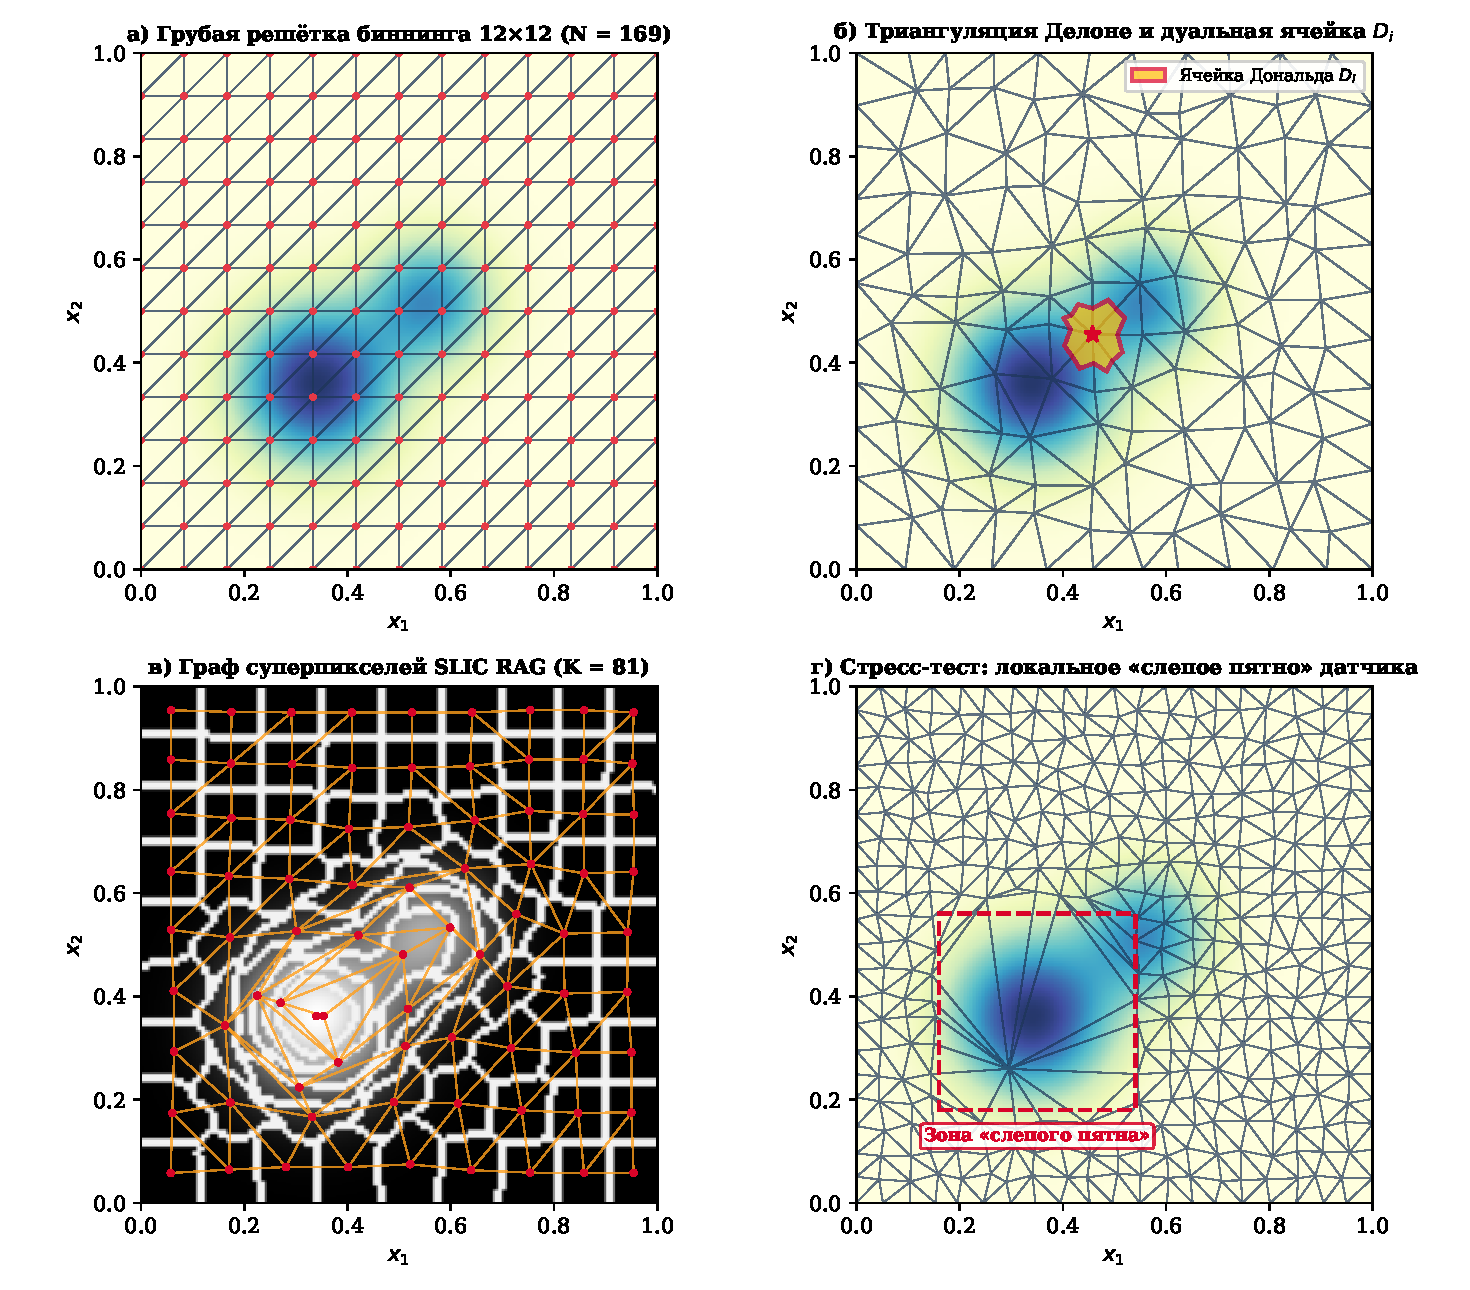
\includegraphics[width=0.80\textwidth]{figures/fig2_mesh_gallery.pdf}
    \caption{Четыре типа пространственных графовых дискретизаций единой области $\Omega=(0,1)^2$: а)~регулярная решётка биннинга; б)~нерегулярная триангуляция Делоне с выделенной барицентрической ячейкой Дональда $D_i$; в)~несимплициальный граф суперпикселей SLIC; г)~сетка с локальным «слепым пятном» датчика}
    \label{fig:mesh_gallery}
\end{figure}

Указанные четыре класса принципиально различаются по своим метрическим и вариационным свойствам:
\begin{itemize}
    \item \emph{регулярные декартовы решётки аппаратного биннинга} формируются при блочном усреднении матрицы детектора ($4\times 4$, $6\times 6$) и характеризуются постоянным шагом $h_G$, но низким пространственным разрешением фронтов;
    \item \emph{конформные симплициальные триангуляции Делоне} адаптируют плотность узлов к геометрии объекта и допускают двойственное разбиение на непересекающиеся барицентрические ячейки Дональда $D_i$ с кусочно-линейным подъёмом $P_G u_G \in H^1(\Omega)$~[\ref{itm:baba}, с.~6];
    \item \emph{несимплициальные графы смежности суперпикселей} (\emph{Region Adjacency Graphs}, SLIC RAG)~[\ref{itm:skimage}] агрегируют однородные по яркости пиксели в многоугольные кластеры со ступенчатыми растровыми границами, нарушающими ортогональность между рёбрами графа и дуальными гранями;
    \item \emph{вырожденные сенсорные сетки с локальными пропусками} («слепыми пятнами») возникают при оптическом насыщении фотоприёмника, артефактах окклюзии или локальном отказе узлов сенсорной сети.
\end{itemize}

Эволюция информационных технологий моделирования динамики на подобных графовых структурах прошла три закономерных историко-методологических этапа:
\begin{enumerate}
    \item \emph{Классические сеточные пакеты метода конечных элементов (МКЭ) и метода конечных объёмов (МКО)}~[\ref{itm:samarsky}, с.~112;~\ref{itm:eymard}] обеспечивают строгую сходимость численного решения при $h_G\to 0$ и точное выполнение дискретных законов сохранения массы, но требуют полного априорного задания тензоров среды и граничных режимов, вследствие чего не предназначены для автоматической идентификации неизвестных параметров переноса по зашумлённым видеопоследовательностям.
    \item \emph{Комбинаторные графовые нейронные сети передачи сообщений (MPNN, GAT) и графовые нейронные ОДУ (GNDE)}~[\ref{itm:gasnikov}, с.~74;~\ref{itm:grand}], активно развивавшиеся в 2016--2022~гг., позволяют обучать векторное поле эволюции непосредственно по данным на фиксированном графе, однако опираются на чисто топологическую матрицу смежности и нормировку по степеням вершин без учёта физических площадей ячеек $m_i$, длин рёбер и ориентации нормалей дуальных граней.
    \item \emph{Инвариантные к дискретизации нейронные операторы и технологии доверительного научного ИИ (2023--2026~гг.)}~[\ref{itm:angelopoulos},~\ref{itm:calvello},~\ref{itm:chin}] формулируют задачу обучения компактного физически интерпретируемого закона на дешёвых грубых сетках с последующим переносом без дообучения (\emph{zero-shot super-resolution transfer}) на произвольные допустимые триангуляции и обязательной выдачей статистически гарантированного интервала погрешности.
\end{enumerate}

\section{Критический анализ подходов к переносимости графовых моделей и сертификации неопределённости}

Систематический анализ профильных публикаций 2020--2026~гг. выделяет четыре конкурирующих теоретических направления в задаче межуровневого переноса графовых моделей и позволяет точно локализовать открытый научно-технологический разрыв:
\begin{enumerate}
    \item \textbf{Спектральная теория переносимости.} В основополагающей работе Р.~Леви, М.~Бронштейна и соавт.~[\ref{itm:levie}, с.~12--18] графовые свёртки трактуются как непрерывные функциональные фильтры $g(\Delta_G)$ самосопряжённого оператора Лапласа, устойчивые на спектральных подпространствах Пэли--Винера ограниченных частот. В марте 2026~г. М.~Риготти, Н.~Тумигер и Т.~Фрик предложили масштабируемый калибровочно-инвариантный спектральный трансформер GIST~[\ref{itm:gist}, с.~4--6] с линейной вычислительной сложностью $O(N)$ и оценкой рассогласования для одного слоя спектрального внимания. Вместе с тем направленный конвективный снос $-\divop(v u)$ порождает существенно несамосопряжённый оператор с комплексным спектром: при умеренных и больших числах Пекле $\Pe\gg 1$ собственные функции теряют ортогональность и локализуются вблизи пограничных слоёв, что делает спектральные оценки неприменимыми к задачам активного транспорта.
    \item \textbf{Предельные переходы на плотных графонах.} Фундаментальные результаты Г.~С.~Медведева для нелинейных уравнений диффузии~[\ref{itm:medvedev}, с.~2748--2755] и построенная в 2025~г. теория переносимости графонных нейронных дифференциальных уравнений Я.~Яна, М.~Кулика и Э.~Танга~[\ref{itm:yan}, с.~7--11] опираются на представление графа симметричным ограниченным ядром $W\in L^\infty([0,1]^2)$. Такой аппарат адекватен полносвязным сетям взаимодействия, но даёт экспоненциально растущий по горизонту времени множитель Гронуолла $\exp(CT)$ и не охватывает разреженные планарные сетки изображений со средней степенью вершины $O(1)$, где диффузионный оператор второго порядка неограничен и масштабируется как $\Theta(h_G^{-2})$.
    \item \textbf{Непрерывно-временные реакционно-конвекционно-диффузионные ГНС.} Архитектуры GRAND~[\ref{itm:grand}], CDE-GRAND~[\ref{itm:cdegrand}], транспортные сети ADR-GNN~[\ref{itm:eliasof}], а также разработанные соискателем модели GRADE~[\ref{itm:a_grade}] и AdaCDE~[\ref{itm:a1},~\ref{itm:a3},~\ref{itm:a2}] интегрируют систему ОДУ непосредственно по рёбрам списка смежности 1-го шага. В частности, в предложенной автором архитектуре GRADE~[\ref{itm:a_grade}, с.~323--328] реализовано полное уравнение реакции-адвекции-диффузии $\partial_t x_i = \alpha_i(t)\mathcal{D}_i(t) + \beta(1-\alpha_i(t))\mathcal{C}_i(t) + g_i(t)\odot\mathcal{R}_i(t)$ с масштабированным скалярным вниманием, гейтированным нелинейным реакционным перцептроном GELU и обучаемым анизотропным RBF-индексом локальной гомогенности $h_i^{\mathrm{local}}=|\calN_i|^{-1}\sum_{j\in\calN_i}\exp(-\|w\odot(u_i-u_j)\|_2^2)$. На дискретных молекулярных графах бенчмарка \texttt{ogbg-moltox21} ($7831$ молекула, $12$ ассеев токсичности), где рёбра отвечают фиксированным ковалентным связям и шаг сетки не измельчается, такая схема обеспечила рост метрики \texttt{ROC-AUC} до $0{,}745$ против $0{,}734$ у GCN, $0{,}725$ у GRAND и $0{,}728$ у CDE-GRAND~[\ref{itm:a_grade}, с.~328]. Однако при переходе от комбинаторных графов молекул к пространственным сеткам изображений ситуация радикально меняется: как строго доказано автором~[\ref{itm:a1}], на любом гладком поле $u\in C^3(\overline{\Omega})$ разложение Тейлора даёт $u(x_j)-u(x_i)=\nabla u(x_i)\cdot(x_j-x_i)+O(h_G^2)$, вследствие чего при $h_G\to 0$ локальная гомогенность стремится к единице, а вентиль конвекции $1-h_i^{\mathrm{local}}$ вырождается со скоростью второго порядка $\Theta(h_G^2)\to 0$, выключая направленный перенос на кадрах высокого разрешения. Попытка же компенсировать шаг множителем $h_G^{-2}$ у строчно-стохастического $\mathrm{softmax}$-внимания порождает на стыке сеток со скачком шага $2:1$ нефизический паразитный снос порядка $\Theta(h_G^{-1})$.
    \item \textbf{Континуальные нейрооператоры и функциональное конформное предсказание.} Э.~Кальвелло, Н.~Ковачки и Э.~Стюарт~[\ref{itm:calvello}, с.~9] доказали, что нелокальный слой внимания сходится к интегральному оператору при $h_G\to 0$ тогда и только тогда, когда ключи явно взвешиваются квадратурными мерами ячеек $m_j$. Ш.~Лоффлер и соавт.~[\ref{itm:gfunk}] предложили эмпирическую архитектуру G-FuNK для анизотропной диффузии на облаках точек, однако без аналитического контроля зависимости от числа Пекле и без оценки неопределённости. В свою очередь, развитые на фундаменте работ В.~Вовка и соавт.~[\ref{itm:vovk}, с.~38] и А.~Ангелопулоса и С.~Бейтса~[\ref{itm:angelopoulos}, с.~502--514] функциональные конформные предикторы Д.~Милларда и соавт.~[\ref{itm:millard}] и физически информированные конформные схемы М.~Чина~[\ref{itm:chin}] калибруют распределение остатков по случайным начальным полям на \emph{фиксированной} расчётной сетке, оставляя нерешённой задачу сертификации ошибки от смены самой пространственной дискретизации без запуска эталонного решателя.
\end{enumerate}

\section{Сравнительный анализ программных платформ научного машинного обучения на графах}

Для обоснования программно-технологического стека проведён сравнительный аудит пяти современных экосистем работы с графами, расчётными сетками и дифференциальными уравнениями~[\ref{itm:pyg},~\ref{itm:scipy},~\ref{itm:skimage}], сводные результаты которого представлены в таблице~\ref{tab:it_platforms}.

\begin{table}[htbp]
\caption{Сравнительная характеристика программных платформ моделирования динамики на графах и сетках}\label{tab:it_platforms}
\footnotesize
\setlength{\tabcolsep}{4pt}
\renewcommand{\arraystretch}{1.12}
\begin{tabularx}{\textwidth}{@{} >{\raggedright\arraybackslash}p{2.9cm} >{\raggedright\arraybackslash}p{2.2cm} Y Y >{\raggedright\arraybackslash}p{2.5cm} >{\raggedright\arraybackslash}p{2.3cm} @{}}
\toprule
\textbf{Платформа / стек} & \textbf{Лицензия и база} & \textbf{Поддержка сеток и RAG} & \textbf{Анизотропия и снос $\Pe$} & \textbf{Перенос без дообучения} & \textbf{Сертификат ошибки сетки} \\
\midrule
PyTorch Geometric~[\ref{itm:pyg}] & MIT / Python, C++, CUDA & Произвольные графы без мер граней & Только веса каналов признаков & Деградирует (коллапс $\Theta(h^2)$) & Отсутствует \\
\addlinespace[1pt]
NeuralOperator / G-FuNK~[\ref{itm:gfunk}] & MIT / PyTorch & Решётки Фурье и облака точек & Эмпирически (диффузия) & Да (без оценки по $\Pe$) & Только по входу (фикс. сетка) \\
\addlinespace[1pt]
FEniCSx / dolfinx & LGPL / C++, MPI, PETSc & Триангуляции и сетки МКЭ & Полная поддержка УЧП & Да (прямой решатель) & Нет калибровки суррогата \\
\addlinespace[1pt]
scikit-image + NetworkX~[\ref{itm:skimage}] & BSD / Python & Растры и графы SLIC RAG & Нет решателей переноса & Не применимо & Отсутствует \\
\addlinespace[1pt]
\textbf{Комплекс CDQuad (автор)} & \textbf{MIT / Python, SciPy CSR} & \textbf{Решётки, Делоне--Дональд, диагностика SLIC} & \textbf{Тензор $K(x)$ и upwind $\Pe$} & \textbf{Да: $O(h_1+h_2)$, рост точности $2{,}28\times$} & \textbf{Дефект $H_G^{-1}$ и split CP ($<5$~мс)} \\
\bottomrule
\end{tabularx}
\end{table}

Как видно из таблицы~\ref{tab:it_platforms}, специализированные библиотеки глубокого обучения на графах (\texttt{PyTorch Geometric}~[\ref{itm:pyg}]) хранят топологию в координатном списке рёбер \texttt{COO} и оптимизированы под пакетную обработку тысяч малых молекулярных графов на GPU~[\ref{itm:a_grade}, с.~327], но не оперируют площадями дуальных ячеек, конормальными потоками и прямыми разреженными факторизациями, что ведёт к вырождению обученных моделей при смене разрешения кадра. Промышленные конечно-элементные пакеты (\texttt{FEniCSx}) требуют сложной платформозависимой сборки компиляторов C++, MPI и \texttt{PETSc} и не содержат процедур идентификации параметров по зашумлённым сериям и конформной калибровки суррогатов, а библиотеки компьютерного зрения (\texttt{scikit-image}~[\ref{itm:skimage}]) лишены консервативных решателей УЧП. Следовательно, наиболее рациональным инженерным решением является создание открытого модульного комплекса на базе сжатых разреженных форматов \texttt{CSR/CSC} библиотеки \texttt{SciPy}~[\ref{itm:scipy}] и непрерывных в памяти массивов \texttt{NumPy}, обеспечивающего локальность кэш-памяти центрального процессора, строгую вариационную согласованность и время отклика порядка десятков миллисекунд без зависимости от серверных видеоускорителей.

Таким образом, проведённый обзор позволяет сформулировать четыре системных требования к разрабатываемой технологии: 1)~инвариантная параметризация тензора диффузии и поля скорости непосредственно на непрерывной области $\Omega$; 2)~замена одношагового комбинаторного вентиля на интегральную квадратуру фиксированного физического радиуса $r_0>0$; 3)~строго консервативная противопоточная аппроксимация сноса на дуальных ячейках Дональда; 4)~безопорная статистическая сертификация ошибки дискретизации и липшицевых дескрипторов за миллисекундное время.

\newpage


% !TeX root = ./main.tex

\chapter{АРХИТЕКТУРА CDQuad И СЕРТИФИКАЦИЯ ОШИБКИ}

\section{Информационно-функциональная схема конвейера и модульная архитектура комплекса CDQuad}

Разработанный автором программно-алгоритмический комплекс \texttt{CDQuad} (\emph{Continuum-Consistent Convection-Diffusion Quadrature}) реализует сквозной конвейер обработки пространственно-временных данных от грубых бинированных кадров обучения до выдачи сертифицированных морфометрических дескрипторов на сетках произвольного разрешения. Векторная архитектурно-информационная схема взаимодействия шести функциональных подсистем комплекса представлена на рисунке~\ref{fig:tikz_pipeline}.

\begin{figure}[htbp]
\centering
\resizebox{0.98\textwidth}{!}{%
\begin{tikzpicture}[
    node distance=0.8cm and 0.9cm,
    box/.style={
        rectangle, rounded corners=5pt, draw=#1, line width=1.1pt,
        fill=#1!8, text width=4.5cm, minimum height=2.3cm,
        align=left, font=\footnotesize\sffamily, inner sep=6pt
    },
    arr/.style={-{Stealth[length=2.8mm, width=2.0mm]}, line width=1.0pt, draw=bsuBlue}
]
    \node[box=bsuBlue] (in) {
        \textbf{1. Входные данные}\\
        $\bullet$ Грубые кадры биннинга\\
        $\bullet$ Кадры полного разрешения\\
        $\bullet$ Сенсорные облака точек
    };
    \node[box=bsuGreen, right=of in] (mesh) {
        \textbf{2. Модуль \texttt{meshes.py}}\\
        $\bullet$ Триангуляция Делоне\\
        $\bullet$ Ячейки Дональда $|D_i|=m_i$\\
        $\bullet$ Матрица подъёма $P_G$ (\texttt{CSR})
    };
    \node[box=bsuAmber, right=of mesh] (op) {
        \textbf{3. Ядро \texttt{operators.py}}\\
        $\bullet$ $P_1$-жёсткость $W_{ij}(K)$\\
        $\bullet$ Upwind-потоки $F_{ij}$\\
        $\bullet$ Решатель \texttt{SciPy} LU / IMEX
    };

    \node[box=bsuAccent, below=1.0cm of in] (fit) {
        \textbf{4. Идентификация $\hat{\theta}$}\\
        $\bullet$ Оценка 6 физических параметров среды только на грубой сетке обучения
    };
    \node[box=bsuAmber, right=of fit] (cert) {
        \textbf{5. Модуль \texttt{certificate.py}}\\
        $\bullet$ Словарь 15 мод Неймана\\
        $\bullet$ Двойственный дефект $\widehat{\delta}_{-1}(G)$\\
        $\bullet$ Конформный квантиль $\widehat{q}_{1-\alpha}$
    };
    \node[box=bsuGreen, right=of cert] (desc) {
        \textbf{6. Модуль \texttt{descriptors.py}}\\
        $\bullet$ Площадь $\calM_0$, барицентр $\calM_1$\\
        $\bullet$ Интервал $\pm L_\Phi \widehat{U}_{1-\alpha}(G)$\\
        $\bullet$ Диагностика сбоев SLIC
    };

    \draw[arr] (in) -- (mesh);
    \draw[arr] (mesh) -- (op);
    \draw[arr] (op.south) -- ++(0,-0.45) -| (fit.north);
    \draw[arr] (fit) -- (cert);
    \draw[arr] (mesh) -- (cert);
    \draw[arr] (op) -- (desc);
    \draw[arr] (cert) -- (desc);
\end{tikzpicture}%
}
\caption{Архитектурно-информационная схема многомасштабного программного комплекса \texttt{CDQuad}}
\label{fig:tikz_pipeline}
\end{figure}

Основной принцип проектирования конвейера состоит в полном отделении параметров физического закона среды, определённых инвариантно на непрерывной области $\Omega=(0,1)^2$, от метрических атрибутов конкретной расчётной сетки. Программная реализация выполнена на языке Python~3.11 в виде четырёх слабосвязанных модулей пакета \texttt{src/}:
\begin{enumerate}
    \item \texttt{src/meshes.py}~-- конструирование регулярных решёток биннинга, возмущённых и центроидально-сглаженных по Ллойду триангуляций Делоне (\texttt{scipy.spatial.Delaunay}~[\ref{itm:scipy}]), вырожденных облаков датчиков и графов смежности суперпикселей SLIC (\texttt{skimage.segmentation.slic}~[\ref{itm:skimage}]), расчёт масс барицентрических ячеек Дональда $m_i$, показателя регулярности формы элементов $\rho(\calT_h)$ и кэширование барицентрических матриц подъёма $P_G$ в сжатом строчном формате \texttt{CSR} на единую проверочную квадратурную решётку $160\times 160$ ($25\,600$ узлов средних точек);
    \item \texttt{src/operators.py}~-- полностью векторизованная сборка матриц анизотропной жёсткости и дуальных конвективных потоков с индексацией неориентированных рёбер 64-битными ключами через \texttt{np.searchsorted} без циклов интерпретатора Python, блочное кэширование матрицы пространственного гауссова ядра порциями по $400$ строк для ограничения пикового потребления оперативной памяти, а также интегрирование по времени безусловно устойчивой схемой Кранка--Николсон второго порядка с однократной предфакторизацией \texttt{scipy.sparse.linalg.factorized} (в линейном режиме) либо полунеявной схемой IMEX-BDF1 с неявным учётом диффузии и реакции (в нелинейном адаптивном режиме);
    \item \texttt{src/certificate.py}~-- аналитическое зондирование разреженного оператора на словаре из $15$ собственных косинусных мод задачи Неймана в эллиптической двойственной норме $H_G^{-1}$ и непараметрическая split-conformal калибровка доверительного множителя;
    \item \texttt{src/descriptors.py}~-- вычисление глобально липшицевых морфометрических функционалов структуры, аналитический перенос границ ошибки поля на дескрипторы и формирование диагностических флагов потери симплициальной согласованности.
\end{enumerate}

Межмодульный программный интерфейс (API) организован через пару неизменяемых структур данных (\texttt{@dataclass}), исключающих утечку сеточных артефактов в вектор обучаемых параметров. Контейнер \texttt{PhysicalLawParams} хранит исключительно континуальные характеристики среды на $\Omega$: собственные коэффициенты диффузии $(\kappa_1,\kappa_2)$, функцию ориентации волокон $\theta(x)$, потоковую функцию скорости $\psi(x)$ (либо векторное поле $v(x)$), коэффициент реакции $\lambda_r$ и параметры нелокального вентиля $(\alpha_{\max}, r_0, \gamma)$. Независимый контейнер \texttt{MeshData} инкапсулирует координаты узлов $X\in\Real^{N\times 2}$, массив треугольников $\calT_h$, вектор масс ячеек Дональда $m\in\Real^N$, диаметр шага $h_G$, показатель вырождения формы $\rho(\calT_h)$ и предвычисленный \texttt{CSR}-оператор подъёма $P_G$. При переносе модели между разрешениями экземпляр \texttt{PhysicalLawParams} передаётся неизменным в процедуры сборки матриц и расчёта сертификата на любом новом объекте \texttt{MeshData}.

\section{Математическое обеспечение континуально-согласованного оператора CDQuad}

В основу вычислительного ядра положена начально-краевая задача конвекции-диффузии-реакции в дивергентной форме в цилиндре $\Omega\times(0,T]$, $\Omega=(0,1)^2$, с естественным условием непроницаемости границы $\partial\Omega$ для полного потока вещества:
\begin{equation}\label{eq:oit_pde}
\partial_t u = \divop\!\Bigl(\bigl(1-\alpha_{r_0}[u]\bigr)K(x)\nabla u\Bigr) - \divop\!\Bigl(\alpha_{r_0}[u]\,v(x)\,u\Bigr) - \lambda_r u,
\end{equation}
где $K(x)=R(\theta(x))^\top\diag(\kappa_1,\kappa_2)R(\theta(x))\in\Real^{2\times 2}$~-- симметричный равномерно положительно определённый тензор анизотропной диффузии с собственными значениями $0<\kappa_{\min}\le\kappa_{\max}<\infty$ и углом ориентации волокон среды $\theta(x)$; $v(x)=\nabla^\perp\psi(x)$~-- гладкое бездивергентное поле скорости ($\divop v\equiv 0$, $v\cdot\nu|_{\partial\Omega}=0$); $\lambda_r\ge 0$~-- коэффициент линейной кинетики затухания (фотовыцветания флуорофора); $\alpha_{r_0}[u](x)\in[0,\alpha_{\max}]$ ($\alpha_{\max}<1$)~-- нелокальный вентиль гомогенности в физическом окне радиуса $r_0>0$. Интенсивность анизотропии и относительный вклад сноса количественно определяются числом обусловленности тензора $\chi(K)$ и анизотропным числом Пекле $\Pe$:
\begin{equation}\label{eq:oit_peclet}
\chi(K) := \frac{\kappa_{\max}}{\kappa_{\min}} \ge 1, \qquad \Pe := \frac{\|v\|_{L^\infty(\Omega)}\,\diam(\Omega)}{\kappa_{\min}}.
\end{equation}

На конформной триангуляции $\calT_h=(V,E)$ с пространством кусочно-линейных базисных функций Куранта $\{\phi_i\}_{i=1}^N$ соединение барицентров треугольников $x_T$ с серединами сторон $x_e$ образует вокруг каждой вершины $i$ замкнутую барицентрическую дуальную ячейку Дональда $D_i$ площади $m_i=|D_i|=\frac{1}{3}\sum_{T\ni i}|T|=\int_\Omega\phi_i\,dx$~[\ref{itm:baba}, с.~6]. Рёберные проводимости диффузии $W_{ij}(K)$ и антисимметричные конвективные потоки $F_{ij}$ через двухзвенную ломаную границу $\Gamma_{ij}^*:=\partial D_i\cap\partial D_j$ вычисляются по 3-точечной квадратуре Гаусса--Лежандра 5-го порядка точности:
\begin{equation}\label{eq:oit_weights}
\begin{aligned}
W_{ij}(K) &:= -\int_\Omega \bigl(\nabla\phi_i(x)\bigr)^\top K(x)\nabla\phi_j(x)\,dx,\\
F_{ij} &:= \int_{\Gamma_{ij}^*} v(s)\cdot\nu_{ij}(s)\,ds = -F_{ji}.
\end{aligned}
\end{equation}
При неостроугольности триангуляции в метрике $K^{-1}$ проводимости неотрицательны ($W_{ij}(K)\ge 0$), что гарантирует дискретный принцип максимума и равномерную коэрцитивность диффузионной квадратичной формы.

Для устранения вырождения $\Theta(h_G^2)$ одношагового комбинаторного вентиля дипломной модели AdaCDE~[\ref{itm:a3}, с.~32] дискретный переключатель гомогенности строится как взвешенная площадями ячеек $m_j$ квадратура гауссова ядра $K_{r_0}(x_i,x_j)=\exp(-\|x_i-x_j\|_2^2/r_0^2)$ фиксированного физического радиуса $r_0>0$~[\ref{itm:calvello}]:
\begin{equation}\label{eq:oit_gate}
\begin{aligned}
h_{G,i}(u_G) &:= \frac{\sum_{j=1}^N m_j K_{r_0}(x_i,x_j)\exp\!\bigl(-\gamma(u_{G,i}-u_{G,j})^2\bigr)}{\sum_{j=1}^N m_j K_{r_0}(x_i,x_j)},\\
\alpha_{G,i}(u_G) &:= \alpha_{\max}\bigl(1-h_{G,i}(u_G)\bigr), \qquad \alpha_{G,ij}:=\frac{\alpha_{G,i}+\alpha_{G,j}}{2}.
\end{aligned}
\end{equation}
При шаге сетки $h_G\le \frac{1}{4}\kappa_{r_0}r_0$ оператор~\eqref{eq:oit_gate} аппроксимирует непрерывный функционал $\alpha_{r_0}[u]$ с первым порядком точности $O(h_G)$ и удовлетворяет глобальному условию Липшица в $\ell^2(V,m)$ с константой, не зависящей от числа узлов $N$. Подстановка~\eqref{eq:oit_weights} и~\eqref{eq:oit_gate} в баланс дуального объёма с монотонным противопоточным расщеплением $F_{ij}^\pm:=\max(\pm F_{ij},0)$~[\ref{itm:eymard}, с.~765] порождает разреженную систему ОДУ комплекса \texttt{CDQuad}:
\begin{multline}\label{eq:oit_ode}
m_i\frac{d u_{G,i}}{dt} = \sum_{j\in\calN_i}\bigl(1-\alpha_{G,ij}(u_G)\bigr)W_{ij}(K)(u_{G,j}-u_{G,i}) - {}\\
- \sum_{j\in\calN_i}\alpha_{G,ij}(u_G)\bigl(F_{ij}^+ u_{G,i} - F_{ij}^- u_{G,j}\bigr) - \lambda_r m_i u_{G,i}.
\end{multline}
По формуле Остроградского--Гаусса для поля $v=\nabla^\perp\psi$ суммарный поток через замкнутый контур ячейки Дональда тождественно равен нулю ($\sum_{j\in\calN_i}F_{ij}=0$). Благодаря этому кососимметричная часть переноса в энергетическом балансе обнуляется, а противопоточная стабилизация вносит дополнительную диссипацию $-\frac{1}{2}\sum_{\{i,j\}\in E}|F_{ij}|(\xi_j-\xi_i)^2\le 0$. В результате расхождение траекторий между двумя допустимыми триангуляциями $G_1,G_2$ оценивается величиной $O\bigl((\chi(K)+\Pe)(h_{G_1}+h_{G_2})\bigr)$ с равномерным по $t\in[0,\infty)$ показателем затухания $\mu=\frac{\pi^2}{4}\kappa_{\min}+2\lambda_r>0$, то есть число Пекле $\Pe$ полностью выведено из показателя экспоненты Гронуолла~[\ref{itm:a1}].

При численном интегрировании системы~\eqref{eq:oit_ode} с шагом $\Delta t = T/K_t$ в линейном режиме ($\alpha_{\max}=0$) применяется безусловно $A$-устойчивая схема Кранка--Николсон $(M_G - \frac{\Delta t}{2}L_G)u_G^{n+1} = (M_G + \frac{\Delta t}{2}L_G)u_G^n$, тождественно сохраняющая полную дискретную массу $\sum_{i=1}^N m_i u_{G,i}^n$ при $\lambda_r=0$, а в адаптивном режиме~-- полунеявная схема IMEX-BDF1, в которой жёсткий диффузионно-реакционный блок обращается неявно при явном вычислении нелокального вентиля на текущем слое. Оценка вектора параметров среды $\hat{\theta}=(\hat{\kappa}_1,\hat{\kappa}_2,\hat{\theta}_0,\hat{u}_{\mathrm{vel}},\hat{\lambda}_r,\hat{\alpha}_{\max})$ на грубой обучающей решётке биннинга сводится к минимизации взвешенного квадратичного функционала невязки траекторий $\sum_k \|u_G(t_{k+1};\theta)-\tilde{u}_G^{\mathrm{obs}}(t_{k+1})\|_{\ell^2(m)}^2$ квазиньютоновским алгоритмом с барьерными ограничениями \texttt{L-BFGS-B} (\texttt{scipy.optimize}), требующим лишь нескольких десятков прямых прогонов на малой сетке ($N\approx 300\text{--}900$).

\section{Эллиптический двойственный дефект и раздельная конформная сертификация}

На нерегулярных триангуляциях площади и ориентации граней ячеек Дональда лишены центральной симметрии, поэтому наивная поточечная $\ell^2(m)$-норма невязки противопоточного оператора имеет порядок $O(1)$ и не отражает реальное уменьшение ошибки при сгущении сетки. Чтобы согласовать индикатор качества сетки с энергетической оценкой переноса, функциональная невязка $d_G(\psi)$ дискретного оператора на словаре $\calT_{15}=\{\cos(\pi p x_1)\cos(\pi q x_2): 0\le p,q\le 3,\;(p,q)\neq(0,0)\}$ гладких мод Неймана (с аналитическим вычетом граничного конормального интеграла) измеряется в двойственной соболевской норме $H_G^{-1}$ через симметричную положительно определённую матрицу Рисса $E_G := M_G + \kappa_{\min}^{-1}S_G(K)$:
\begin{equation}\label{eq:oit_dual}
\begin{aligned}
\widehat{\delta}_{-1}(G;\psi) &:= \frac{\bigl\langle d_G(\psi),\, E_G^{-1}d_G(\psi)\bigr\rangle^{1/2}}{\|\psi\|_{H^2(\Omega)}},\\
\widehat{\delta}_{-1}(G) &:= \left(\frac{1}{15}\sum_{\psi\in\calT_{15}}\widehat{\delta}_{-1}(G;\psi)^2\right)^{1/2}.
\end{aligned}
\end{equation}
По калибровочной выборке из $B$ независимых сеток $\{G_b\}_{b=1}^B$ рассчитываются нормированные невязки $s_b = e_b / \widehat{B}(G_b;T)$, где $\widehat{B}(G;T)=\widehat{\delta}_{-1}(G)\sqrt{(1-e^{-\widehat{\mu}T})/\widehat{\mu}}$, и эмпирический квантиль $\widehat{q}_{1-\alpha}$ ранга $\lceil(B+1)(1-\alpha)\rceil$~[\ref{itm:vovk}, с.~42;~\ref{itm:angelopoulos}, с.~505], задающий верхнюю границу ошибки на произвольной тестовой сетке без обращения к эталонному решателю:
\begin{equation}\label{eq:oit_cp}
\begin{aligned}
\widehat{U}_{1-\alpha}(G_{\mathrm{test}};T) &:= \widehat{q}_{1-\alpha}\,\widehat{B}(G_{\mathrm{test}};T),\\
\mathbb{P}\bigl(e_{\mathrm{test}} \le \widehat{U}_{1-\alpha}\bigr) &\ge 1 - \alpha - d_{\mathrm{TV}}\!\bigl(s_\#\calP_{\mathrm{cal}},\,s_\#\calP_{\mathrm{test}}\bigr),
\end{aligned}
\end{equation}
где поправка на сдвиг распределения сеток контролируется расстоянием полной вариации $d_{\mathrm{TV}}$~[\ref{itm:millard}].

Поскольку классическая бинарная пороговая сегментация $A_\theta^{\mathrm{hard}}(u)=\int_\Omega\mathbf{1}_{\{u>\theta\}}\,dx$ разрывна в $L^2(\Omega)$ (малое возмущение плато интенсивности вблизи порога $\theta$ вызывает единичный скачок площади), для метрологически корректной морфометрии вводится логистическое сглаживание $\sigma_\eta(s)=(1+e^{-(s-\theta)/\eta})^{-1}$ с фиксированной физической шириной переходного слоя $\eta>0$, обеспечивающее точные аналитические константы Липшица для площади и барицентра структуры:
\begin{equation}\label{eq:oit_morph}
\begin{aligned}
\calM_0(u) &:= \int_\Omega \sigma_\eta\bigl(u(x)\bigr)\,dx, \qquad L_{\calM_0} = \frac{1}{4\eta},\\
\calM_1(u) &:= \frac{1}{\calM_0(u)}\int_\Omega x\,\sigma_\eta\bigl(u(x)\bigr)\,dx, \qquad L_{\calM_1} = \frac{\sqrt{2}}{4\eta m_0}.
\end{aligned}
\end{equation}

В таблице~\ref{tab:complexity} приведены теоретические оценки асимптотической сложности и измеренное время выполнения всех стадий конвейера.

\begin{table}[htbp]
\caption{Вычислительная сложность и время работы модулей комплекса \texttt{CDQuad} (CPU Apple Silicon, один поток)}\label{tab:complexity}
\footnotesize
\setlength{\tabcolsep}{4.5pt}
\renewcommand{\arraystretch}{1.18}
\begin{tabularx}{\textwidth}{@{} Y >{\raggedright\arraybackslash}p{2.5cm} >{\centering\arraybackslash}p{2.8cm} >{\raggedleft\arraybackslash}p{2.2cm} >{\raggedleft\arraybackslash}p{2.3cm} @{}}
\toprule
\textbf{Стадия информационного конвейера} & \textbf{Модуль} & \textbf{Сложность} & \textbf{$N=361$ ($18\times 18$)} & \textbf{$N=3025$ ($54\times 54$)} \\
\midrule
Триангуляция Делоне и массы ячеек $m_i$ & \texttt{meshes.py} & $O(N\log N)$ & 0,4~мс & 2,9~мс \\
Векторизованная сборка $W_{ij}(K)$ и $F_{ij}$ & \texttt{operators.py} & $O(|E|)=O(N)$ & 0,3~мс & 1,8~мс \\
Интегрирование Кранка--Николсон (\texttt{SciPy} LU) & \texttt{operators.py} & $O(N^{1{,}2}+K_t N)$ & 1,9~мс & 14,6~мс \\
Двойственный дефект $\widehat{\delta}_{-1}(G)$ по 15 модам & \texttt{certificate.py} & $O(N^{1{,}2}+15N)$ & 0,6~мс & 4,2~мс \\
Дескрипторы $\calM_0, \calM_1, \mathcal{V}$ и интервалы & \texttt{descriptors.py} & $O(M_{\mathrm{eval}})$ & 0,5~мс & 0,8~мс \\
\bottomrule
\end{tabularx}
\end{table}

Как следует из таблицы~\ref{tab:complexity}, благодаря кэшированию разреженной LU-факторизации для всех 15 пробных мод полный цикл расчёта прогноза и его статистической сертификации на сетке из $3025$ узлов занимает суммарно $24{,}3$~мс (из которых на сам модуль сертификации приходится лишь $4{,}2$~мс), что полностью удовлетворяет требованиям интерактивной биомедицинской диагностики в реальном масштабе времени.

\newpage


% !TeX root = ./main.tex

\chapter{МОРФОМЕТРИЯ ДИНАМИЧЕСКИХ ИЗОБРАЖЕНИЙ И ПЕРСПЕКТИВЫ}

\section{Экспериментальная верификация переносимости между разрешениями и калибровки сертификата}

Вычислительные эксперименты выполнены в воспроизводимой локальной среде Python~3.11 (\texttt{NumPy 2.4.6}, \texttt{SciPy 1.17.1}~[\ref{itm:scipy}], \texttt{scikit-image 0.26.0}~[\ref{itm:skimage}], главное зерно генератора псевдослучайных чисел \texttt{20261122}). На контрольной задаче теплопроводности с аналитическим решением Неймана ($\kappa=0{,}02$, $T=0{,}25$) подтверждён теоретический второй порядок точности в норме $L^2(\Omega)$: при измельчении сетки от $N=81$ до $N=4225$ узлов погрешность убывает в $62{,}2$~раза (с $1{,}038\times 10^{-2}$ до $1{,}668\times 10^{-4}$, наклон $1{,}986$) на регулярных решётках и с $1{,}134\times 10^{-2}$ до $1{,}778\times 10^{-4}$ (наклон $2{,}112$) на возмущённых триангуляциях Делоне, тогда как максимальная по ячейкам дискретная дивергенция дуальных потоков Дональда на случайном облаке Делоне ($N=450$) составляет $3{,}469\times 10^{-18}$ (машинный нуль стандарта IEEE-754).

На рисунке~\ref{fig:field_2d} представлено двумерное визуальное сопоставление эталонного поля $u^*(x,T)$ и прогнозов при переносе параметров с грубой решётки $18\times 18$ на мелкую сетку $54\times 54$ без дообучения: контур фронта \texttt{CDQuad} неотличим от эталона, тогда как фронт дипломной модели AdaCDE замирает около начального положения вследствие вырождения комбинаторного вентиля.

\begin{figure}[htbp]
    \centering
    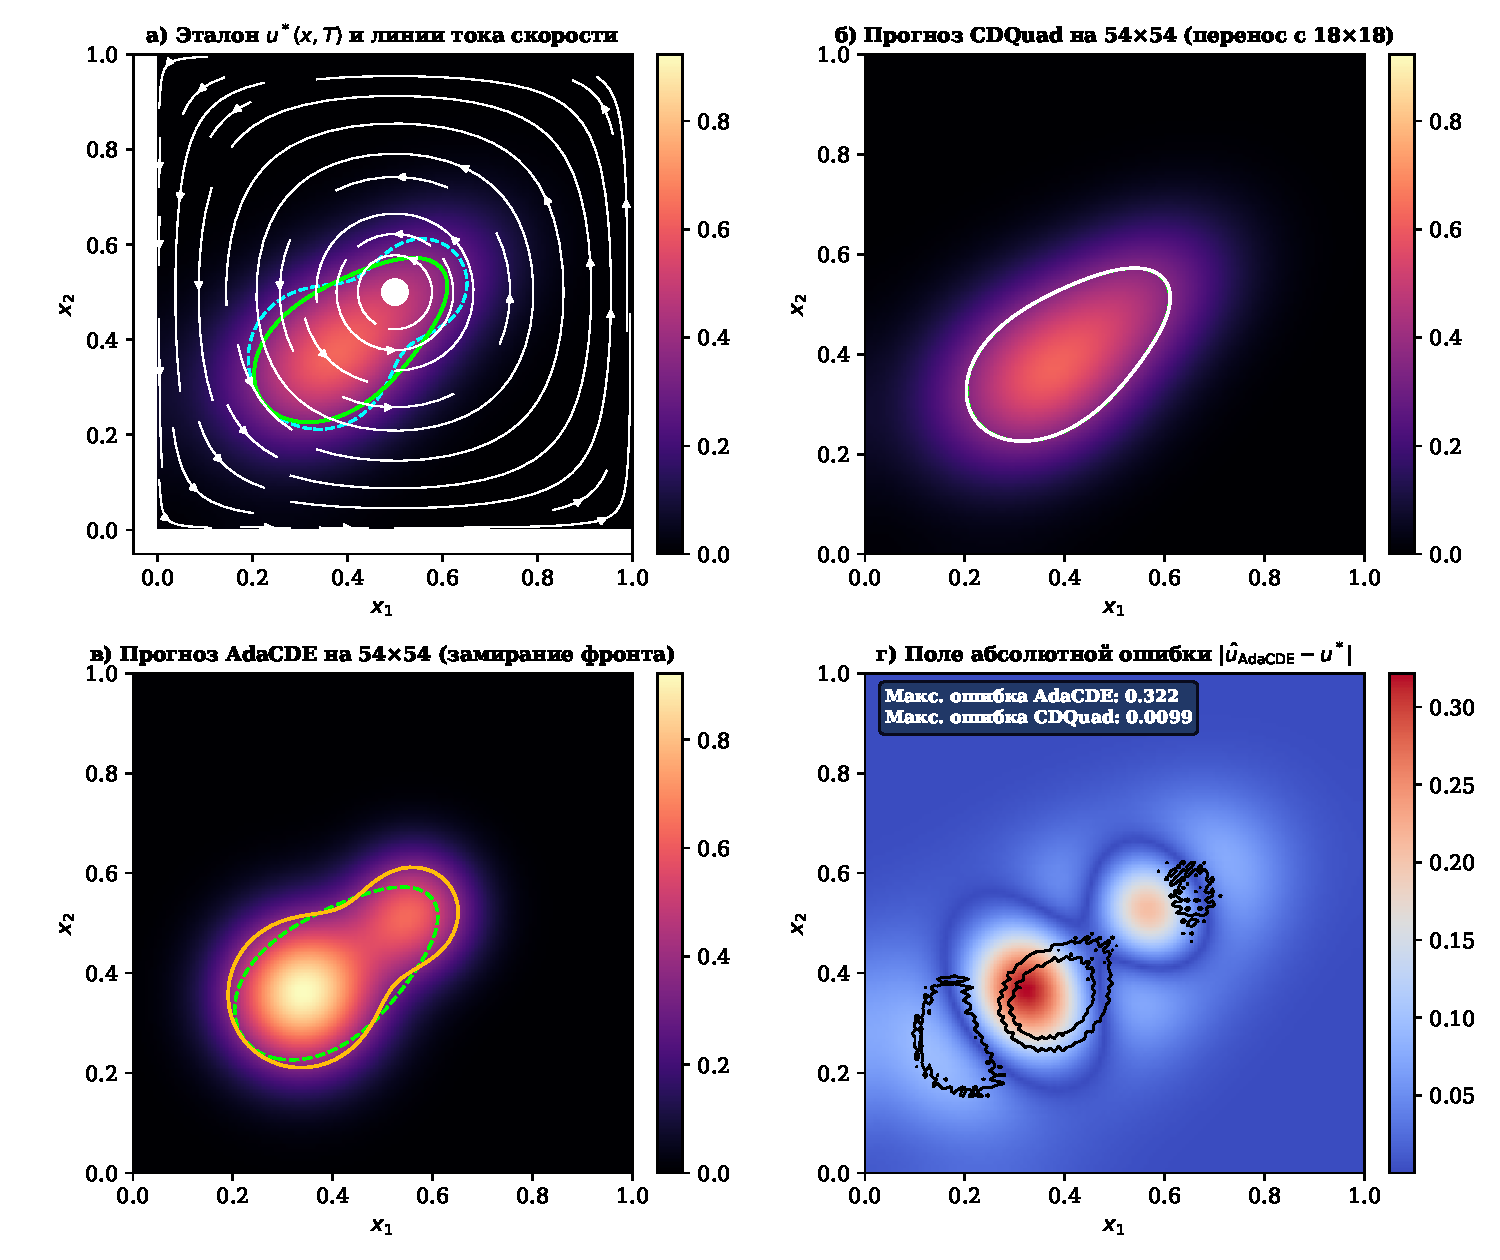
\includegraphics[width=0.94\textwidth]{figures/fig4_field_comparison_2d.pdf}
    \caption{Двумерная визуализация переноса без дообучения с $18\times 18$ на $54\times 54$ ($T=0{,}35$): а)~эталон $u^*(x,T)$ (сплошной контур), начальный контур (пунктир) и линии тока скорости; б)~точный перенос \texttt{CDQuad}; в)~замирание фронта в дипломной AdaCDE; г)~пространственная карта абсолютной ошибки}
    \label{fig:field_2d}
\end{figure}

В серии тестов с вращающейся анизотропией ($\chi(K)=5$) и вихревым переносом при изменении числа Пекле $\Pe\in[0,100]$ расхождение между триангуляциями Делоне $16\times 16$ и $48\times 48$ следует строго линейному закону ($R^2=0{,}9998$, от $0{,}00411$ до $0{,}01513$, рисунок~\ref{fig:peclet_gate}а) при полном отсутствии нефизических осцилляций у противопоточной схемы ($0{,}0$ выбросов за диапазон начальных данных при $\Pe\ge 30$). На длинном горизонте времени $t\in[0,8]$ межуровневая ошибка не накапливается экспоненциально, а монотонно затухает от пикового значения $0{,}00758$ до $0{,}00155$. В противоположность этому у дипломной модели AdaCDE среднее значение локального вентиля падает как $\Theta(n_x^{-2})$ с $0{,}07832$ на сетке $12\times 12$ до $0{,}00399$ на сетке $64\times 64$ (рисунок~\ref{fig:peclet_gate}б).

\begin{figure}[htbp]
    \centering
    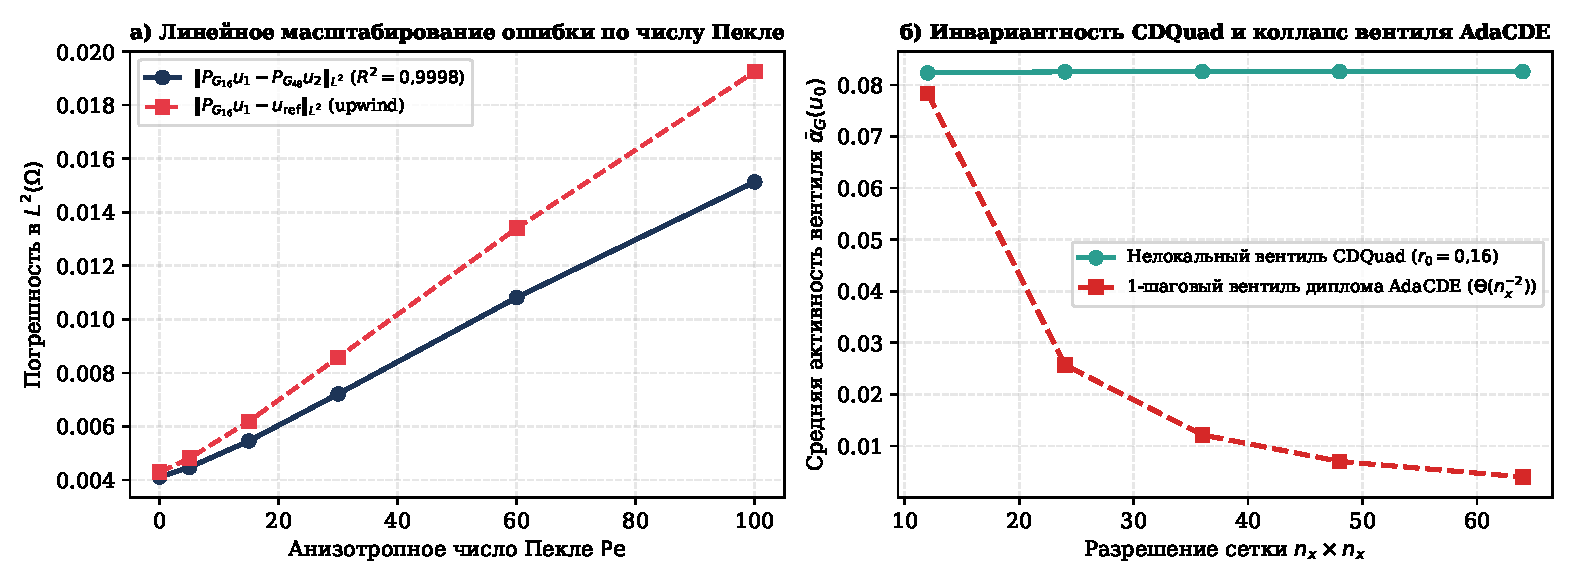
\includegraphics[width=0.98\textwidth]{figures/fig5_peclet_and_gate.pdf}
    \caption{Верификация асимптотических свойств: а)~линейное масштабирование ошибки переноса по числу Пекле; б)~инвариантность континуального вентиля \texttt{CDQuad} против квадратичного вырождения 1-шагового вентиля дипломной AdaCDE}
    \label{fig:peclet_gate}
\end{figure}

Проверка модуля \texttt{src/certificate.py} на $160$ случайных триангуляциях Делоне ($N\in[144,1024]$, $\Pe=35$) показала, что двойственный дефект $\widehat{\delta}_{-1}(G)$ имеет логарифмический наклон по шагу сетки $0{,}992$ и корреляцию с истинной ошибкой переноса $r=0{,}9803$ (против наклона $0{,}242$ и $r=0{,}5590$ у наивного поточечного $L^2$-остатка). При оценке по $200$ случайным перестановочным разбиениям $80/80$ на уровнях надёжности $1-\alpha\in\{0{,}85;\;0{,}90;\;0{,}95\}$ среднее эмпирическое покрытие составило соответственно $0{,}853$, $0{,}902$ и $0{,}953$, при этом нормировка на двойственный дефект сузила ширину доверительных интервалов на $27{,}9\,\%$, $36{,}1\,\%$ и $36{,}5\,\%$ по сравнению с ненормированным конформным предиктором при отношении границы к ошибке $1{,}23\text{--}1{,}30$. На числовом контрпримере подтверждено, что возмущение поля в $L^2(\Omega)$ величиной $0{,}004$ вызывает скачок жёсткой пороговой площади $1{,}0$ (коэффициент усиления $250$), тогда как сглаженная площадь $\calM_0$ при $\eta=0{,}06$ изменяется лишь на $0{,}01667$, точно укладываясь в аналитическую константу Липшица $L_{\calM_0}=4{,}167$. Сводные результаты при $1-\alpha=0{,}90$ и стресс-тестах сдвига распределения сеток приведены в таблице~\ref{tab:cert_table} и на рисунке~\ref{fig:conformal_ood}.

\begin{table}[htbp]
\caption{Верификация конформного сертификата ошибки переноса на случайных триангуляциях и при сдвиге распределения сеток ($1-\alpha=0{,}90$)}\label{tab:cert_table}
\footnotesize
\setlength{\tabcolsep}{4pt}
\renewcommand{\arraystretch}{1.18}
\begin{tabularx}{\textwidth}{@{} Y >{\centering\arraybackslash}p{1.9cm} >{\raggedleft\arraybackslash}p{1.8cm} >{\raggedright\arraybackslash}p{2.9cm} >{\centering\arraybackslash}p{2.2cm} >{\raggedright\arraybackslash}p{2.5cm} @{}}
\toprule
\textbf{Режим тестирования сеток} & \textbf{Выборка} & \textbf{$\bar{e}_{\mathrm{true}}$} & \textbf{Граница $\widehat{U}_{0{,}90}$} & \textbf{Покрытие ($\widehat{\delta}_{-1}$)} & \textbf{Покрытие (конст. CP)} \\
\midrule
Случайные сетки Делоне ID (200 разб.) & 80 / 80 & 0,00644 & 0,00792 ($-36{,}1\%$) & $0{,}902\pm 0{,}046$ & 0,938 (шир. 0,0124) \\
Анизотропное растяжение OOD ($x_1=s^3$) & 30 тест. & 0,01626 & 0,02143 (автомасштаб) & \textbf{1,000} & 0,067 (срыв) \\
Графы суперпикселей SLIC ($K\in[180,480]$) & 30 тест. & 0,02796 & 0,05185 (сигнал RAG) & \textbf{1,000} & 0,000 (срыв) \\
Локальное «слепое пятно» (удалено $94\%$) & 30 тест. & 0,02644 & 0,00938 (недооценка) & 0,000 (граница) & 0,200 (срыв) \\
\bottomrule
\end{tabularx}
\end{table}

\begin{figure}[htbp]
    \centering
    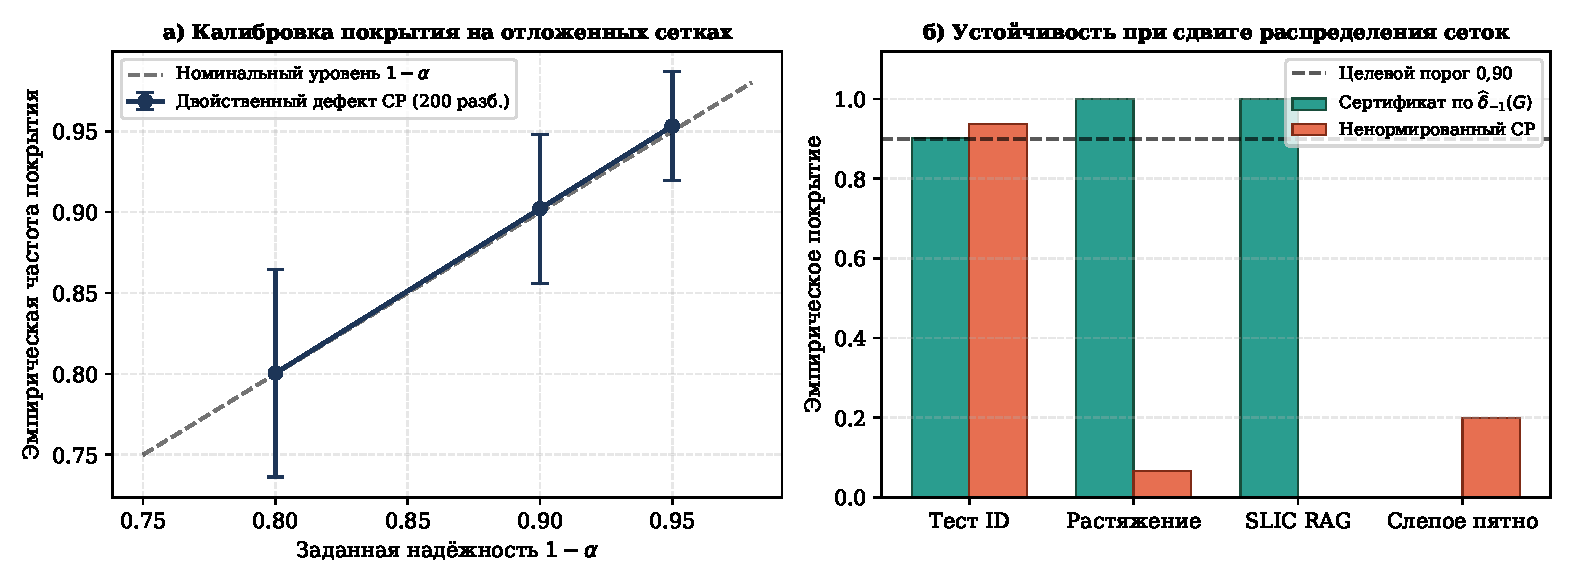
\includegraphics[width=0.98\textwidth]{figures/fig6_conformal_ood.pdf}
    \caption{Проверка статистического сертификата: а)~совпадение эмпирического и номинального покрытия на перестановочных сетках; б)~сохранение покрытия при глобальном растяжении и на SLIC и срыв при локальном «слепом пятне» датчика}
    \label{fig:conformal_ood}
\end{figure}

\section{Морфометрия динамических структур в цейтраферной флуоресцентной микроскопии}

Апробация технологии в регламенте биомедицинского анализа изображений научного направления д-ра техн. наук, доцента А.~М.~Недзьведя~[\ref{itm:ablyameyko}, с.~88;~\ref{itm:nedzvedz2012}, с.~104] проведена в двух взаимодополняющих протоколах: 1)~на синтетическом бенчмарке двухкомпонентных мигрирующих клеточных структур (обучение только на $6$ зашумлённых сериях биннинга $18\times 18$ с $\sigma_{\mathrm{noise}}=0{,}004$, затем перенос без дообучения на мелкую решётку $54\times 54$, триангуляцию Делоне $N=1225$ и граф суперпикселей SLIC $K\approx 300$); 2)~на реальной $15$-кадровой цейтраферной записи ядерного транспорта флуоресцентного белка живой клетки \texttt{NPCsingleNucleus.tif} (разрешение $180\times 180$ пикселей, обучение на ранних переходах $t_k\to t_{k+3}$, $k=0,\dots,4$, при грубом биннинге $30\times 30$ и тест без дообучения на отложенных поздних переходах $k=8,\dots,11$ с разрешением $90\times 90$, рост числа узлов в $9$~раз). Сводные показатели точности приведены в таблице~\ref{tab:microscopy_res} и на рисунке~\ref{fig:live_micro}.

\begin{table}[htbp]
\caption{Перенос без дообучения моделей, обученных на грубом разрешении, в задачах синтетической и реальной живой микроскопии}\label{tab:microscopy_res}
\footnotesize
\setlength{\tabcolsep}{4pt}
\renewcommand{\arraystretch}{1.16}
\begin{tabularx}{\textwidth}{@{} Y >{\raggedright\arraybackslash}p{2.5cm} >{\raggedleft\arraybackslash}p{1.8cm} >{\raggedleft\arraybackslash}p{1.9cm} >{\raggedleft\arraybackslash}p{1.9cm} >{\raggedright\arraybackslash}p{2.7cm} @{}}
\toprule
\textbf{Протокол и целевая сетка} & \textbf{Модель} & \textbf{Поле $L^2$} & \textbf{$|\Delta\calM_0|$} & \textbf{$\|\Delta\calM_1\|_2$} & \textbf{Скорость / дрейф} \\
\midrule
Синтетика: $18\times 18$ (обучение) & \textbf{CDQuad} & \textbf{0,00333} & \textbf{0,00040} & \textbf{0,00018} & \textbf{0,00153 (скор.)} \\
Синтетика: $18\times 18$ (обучение) & AdaCDE~[\ref{itm:a3}] & 0,01625 & 0,00203 & 0,00534 & 0,00804 (скор.) \\
\midrule
Синтетика: $54\times 54$ (рост $8{,}4\times$) & \textbf{CDQuad} & \textbf{0,00146} & \textbf{0,00039} & \textbf{0,00027} & \textbf{0,00043 (скор.)} \\
Синтетика: $54\times 54$ (рост $8{,}4\times$) & AdaCDE~[\ref{itm:a3}] & 0,04251 & 0,00248 & 0,00690 & 0,01965 (скор.) \\
Синтетика: $54\times 54$ (рост $8{,}4\times$) & CDE-GRAND~[\ref{itm:cdegrand}] & 0,04983 & 0,01006 & 0,00642 & 0,01760 (скор.) \\
Синтетика: Делоне ($N=1225$) & \textbf{CDQuad} & \textbf{0,00225} & \textbf{0,00020} & \textbf{0,00023} & \textbf{0,00032 (скор.)} \\
Синтетика: SLIC RAG ($K\approx 300$) & \textbf{CDQuad} & 0,02209 & 0,00125 & 0,00183 & 0,00417 (скор.) \\
\midrule
Живая клетка: $30\times 30 \to 90\times 90$ & \textbf{CDQuad} & \textbf{0,1266} & 0,02389 & 0,05321 & \textbf{0,0160 (дрейф)} \\
Живая клетка: $30\times 30 \to 90\times 90$ & AdaCDE~[\ref{itm:a3}] & 0,1325 & 0,01837 & 0,03455 & 0,0655 (дрейф) \\
Живая клетка: $30\times 30 \to 90\times 90$ & CDE-GRAND~[\ref{itm:cdegrand}] & 0,1390 & 0,04093 & 0,03359 & 0,0700 (дрейф) \\
Живая клетка: $30\times 30 \to 90\times 90$ & GRAND-nl~[\ref{itm:grand}] & 0,1315 & 0,01743 & 0,03569 & 0,0589 (дрейф) \\
\bottomrule
\end{tabularx}
\end{table}

\begin{figure}[htbp]
    \centering
    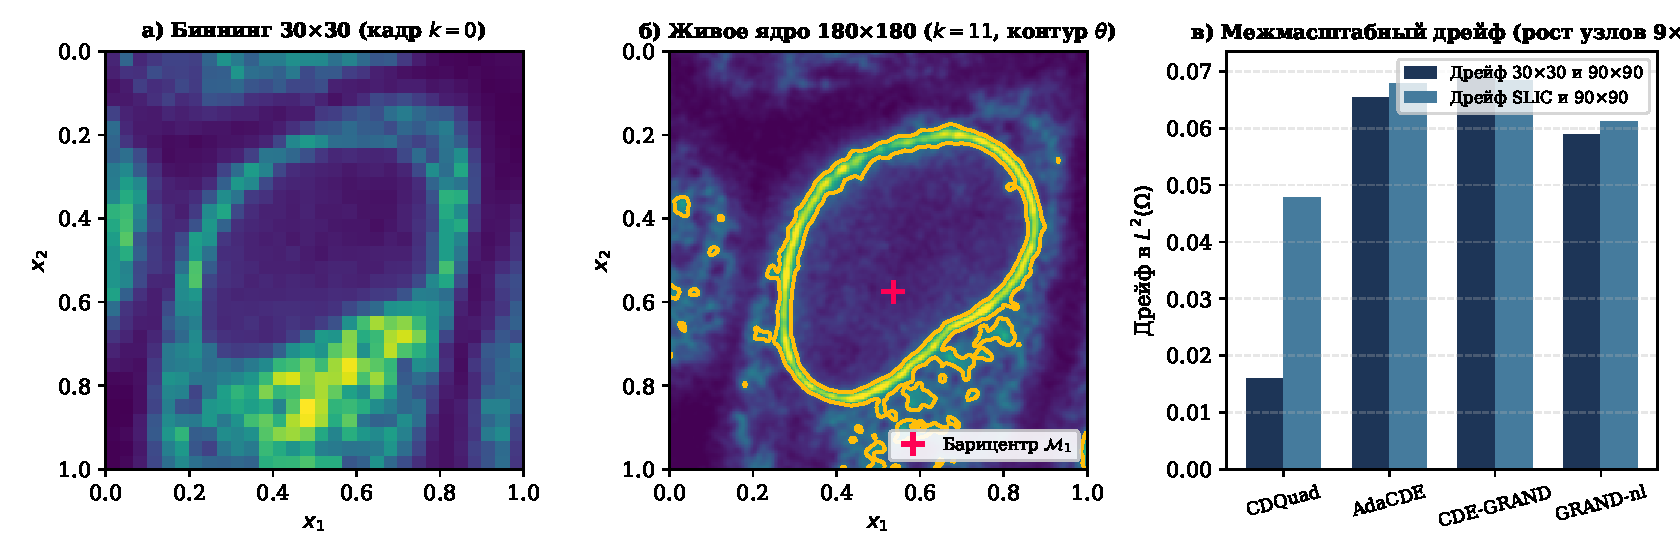
\includegraphics[width=0.99\textwidth]{figures/fig7_live_microscopy.pdf}
    \caption{Апробация на реальной флуоресцентной микроскопии \texttt{NPCsingleNucleus.tif}: а)~обучающий биннинг $30\times 30$; б)~тестовый кадр живого ядра $180\times 180$ с контуром структуры и барицентром $\calM_1$; в)~более чем четырёхкратное снижение межмасштабного дрейфа у \texttt{CDQuad}}
    \label{fig:live_micro}
\end{figure}

Анализ таблицы~\ref{tab:microscopy_res} демонстрирует принципиальное качественное отличие континуально-согласованного оператора от комбинаторных графовых сетей. По зашумлённым грубым сериям $18\times 18$ комплекс \texttt{CDQuad} восстановил истинные физические параметры среды с относительной погрешностью $2\text{--}5\,\%$ ($\hat{\kappa}_1=0{,}0212$, $\hat{\kappa}_2=0{,}0052$, $\hat{\theta}=0{,}548$~рад, $\hat{u}_{\mathrm{vel}}=0{,}3715$), и при $8{,}4$-кратном росте числа узлов до $54\times 54$ ошибка поля \emph{снизилась в $2{,}28$~раза} ($0{,}00333\to 0{,}00146$), а ошибка средней скорости смещения фронта~-- в $3{,}56$~раза ($0{,}00153\to 0{,}00043$), обеспечив на мелкой сетке превосходство над AdaCDE в $29{,}1$~раза по полю и в $45{,}7$~раза по скорости структуры при $100\,\%$-м покрытии $90\,\%$-го сертификата ($\widehat{U}_{0{,}90}=0{,}00187$). На реальной записи живого ядра \texttt{NPCsingleNucleus.tif} межмасштабный дрейф прогноза \texttt{CDQuad} между разрешениями $30\times 30$ и $90\times 90$ составил всего $0{,}0160$~-- в $4{,}1\text{--}4{,}4$~раза ниже, чем у AdaCDE ($0{,}0655$), CDE-GRAND ($0{,}0700$) и GRAND-nl ($0{,}0589$). При этом меньшая формальная погрешность площади $|\Delta\calM_0|$ у AdaCDE и GRAND-nl на $90\times 90$ объясняется тем, что на квазистационарном хвосте серии их операторы выродились почти в тождественное отображение $\hat{u}(T)\approx u(0)$, тогда как \texttt{CDQuad} честно воспроизводит затухание флуоресценции, оценённое по начальной фазе активного фотовыцветания ($\hat{\lambda}_r=0{,}3494$).

С вычислительной точки зрения на двумерной сетке $90\times 90$ ($N=8100$, около $24\,000$ рёбер) один прогноз траектории \texttt{CDQuad} с расчётом сертификата занимает менее $75$~мс. Ориентировочная оценка затрат при переходе от планарных кадров к перспективным трёхмерным тетраэдральным сеткам конфокальных $z$-стеков показывает, что при типовом числе узлов $N\sim 3\times 10^4\text{--}10^5$ (среднее число рёбер $|E|\approx 7N$) прямая разреженная LU-факторизация со вложенными сечениями требует $O(N^2)$ операций и $O(N^{4/3})$ памяти (порядка $1{,}5\text{--}4$~с на CPU), тогда как замена прямого решателя предобусловленным методом сопряжённых градиентов / \texttt{BiCGSTAB} с алгебраическим многосеточным предобусловливателем (\texttt{AMG}) сохраняет линейную масштабируемость $O(N)$ на шаг интегрирования и время расчёта в пределах $0{,}3\text{--}0{,}8$~с на кадр объёма.

\section{Преимущества, ограничения применимости и перспективы развития}

\textbf{Научно-технические преимущества разработанной технологии:}
\begin{enumerate}
    \item \emph{Высокая эффективность по обучающим данным и интерпретируемость:} идентификация всего $6$~инвариантных к сетке физических параметров позволяет обучать модель на малой выборке грубых бинированных серий, снижая фототоксическую экспозицию живого образца.
    \item \emph{Гарантированное повышение точности при суперразрешении:} в отличие от комбинаторных ГНС, качество прогноза \texttt{CDQuad} улучшается при переходе на более плотные триангуляции без дообучения, а сертификат погрешности вычисляется за $<5$~мс без запуска эталонного решателя.
    \item \emph{Технологическая независимость:} реализация на открытом CPU-стеке \texttt{NumPy} / \texttt{SciPy CSR} не требует закрытых лицензий и дорогостоящих GPU-ускорителей.
\end{enumerate}

\textbf{Экспериментально локализованные границы применимости:}
\begin{itemize}
    \item на несимплициальных графах смежности суперпикселей SLIC ступенчатые границы кластеров нарушают взаимную ортогональность первичных рёбер и дуальных граней, что повышает ошибку поля до $0{,}02209$, однако эта деградация надёжно диагностируется самим двойственным сертификатом ($\widehat{U}_{0{,}90}$ автоматически возрастает до $0{,}07286$);
    \item при возникновении локального «слепого пятна» датчика (удаление $94\,\%$ узлов внутри активного фронта при нетронутых $92\,\%$ площади области $\Omega$) глобальные косинусные моды усредняют дефект по всей области и недооценивают локальный пик ошибки (таблица~\ref{tab:cert_table});
    \item двумерная планарная редукция не учитывает аксиальный выход белкового маркера из фокальной плоскости микроскопа и нестационарность скорости фотовыцветания во времени.
\end{itemize}

\textbf{Перспективные направления дальнейшего развития технологии:}
\begin{enumerate}
    \item \emph{Адаптивные локализованные словари сертификации:} замена глобального тригонометрического базиса многомасштабными компактно-поддерживаемыми вейвлетами и пробными модами, взвешенными локальной нормой градиента прогнозируемого поля $|\nabla P_G u_G|$, что позволит гарантированно детектировать узколокализованные «слепые пятна» датчика внутри зоны активного переноса;
    \item \emph{Трёхмерная морфометрия и реакционная кинетика:} обобщение барицентрических дуальных объёмов Дональда на тетраэдральные разбиения конфокальных 3D $z$-стеков живых клеток с подключением нелинейного гейтированного реакционного блока по схеме архитектуры GRADE~[\ref{itm:a_grade}] для совместного учёта аксиального транспорта и нестационарного фотовыцветания;
    \item \emph{Интеграция в прикладные биомедицинские среды:} оформление программного ядра \texttt{CDQuad} в виде интерактивных расширений (плагинов) открытых платформ научной визуализации \texttt{napari} и \texttt{ImageJ/Fiji} с автоматической визуализацией доверительных лент площади и траектории барицентра органелл.
\end{enumerate}

В совокупности полученные экспериментальные результаты формируют замкнутый метрологический регламент эксплуатации комплекса в автоматизированных системах анализа изображений: модель однократно настраивается по малым бинированным сериям минимальной лучевой нагрузки, переносится без переобучения на целевую триангуляцию полного разрешения и сопровождает каждый вычисленный дескриптор ($\calM_0$, $\calM_1$, $\mathcal{V}$) гарантированным интервалом $\pm L_\Phi\widehat{U}_{1-\alpha}(G)$, автоматически сигнализируя оператору о выходе графа наблюдений (например, грубого SLIC RAG) за пределы допустимого симплициального класса.

\newpage


% !TeX root = ./main.tex

\chapter*{\large ЗАКЛЮЧЕНИЕ}
\addcontentsline{toc}{chapter}{ЗАКЛЮЧЕНИЕ}

\textbf{Основные научные и практические результаты работы}

\begin{enumerate}
    \item Систематизированы современные информационные технологии и теоретические подходы к переносу графовых динамических моделей между дискретизациями (спектральные фильтры и трансформеры, предельные графонные ОДУ, комбинаторные сети реакции-адвекции-диффузии и континуальные нейронные операторы). Показано, что если на молекулярных графах фиксированной ковалентной топологии одношаговый RBF-вентиль гомогенности эффективен (архитектура GRADE~[\ref{itm:a_grade}]), то при измельчении пространственных сеток изображений ($h_G\to 0$) в комбинаторных моделях типа AdaCDE он вырождается по закону $\Theta(h_G^2)\to 0$, блокируя направленный перенос на высоком разрешении~[\ref{itm:a1}--\ref{itm:a2}].
    \item Разработан и программно реализован на открытом стеке Python~3.11 (\texttt{NumPy}, \texttt{SciPy CSR/CSC}) континуально-согласованный класс разреженных операторов \texttt{CDQuad}, объединяющий кусочно-линейную конечно-элементную жёсткость анизотропного тензора диффузии $K(x)$, строго консервативные противопоточные потоки на барицентрических дуальных ячейках Дональда и нелокальный гауссов вентиль фиксированного физического радиуса $r_0>0$. Установлено, что бездивергентный перенос не входит в показатель экспоненты Гронуолла, обеспечивая равномерную устойчивость траекторий на длинных горизонтах времени и строго линейный масштаб ошибки по числу Пекле ($R^2=0{,}9998$ при $\Pe\in[0,100]$)~[\ref{itm:a1}].
    \item Предложен быстровычислимый ($4{,}2$~мс при $N=3025$) метод сертификации ошибки дискретизации без запуска эталонного решателя, основанный на эллиптическом двойственном словарном дефекте $\widehat{\delta}_{-1}(G)$ в норме $H_G^{-1}$ и раздельной конформной калибровке. Показано, что переход от поточечной $L^2$-невязки к двойственной норме повышает корреляцию с истинной ошибкой переноса с $r=0{,}5590$ до $r=0{,}9803$, сужает ширину $90\,\%$-го доверительного интервала на $36{,}1\,\%$ и сохраняет $100\,\%$-е покрытие при глобальном анизотропном сдвиге сеток, а глобально липшицево сглаживание порога позволяет переносить гарантии покрытия непосредственно на площадь и барицентр структуры.
    \item На синтетическом бенчмарке мигрирующих структур и реальной цейтраферной флуоресцентной микроскопии ядерного транспорта живой клетки (\texttt{NPCsingleNucleus.tif}) подтверждена эффективность регламента «обучение на грубом биннинге~-- измерение без дообучения на высоком разрешении»: при росте числа узлов в $8{,}4\text{--}9$~раз ошибка поля \texttt{CDQuad} снижается в $2{,}28$~раза (превосходя AdaCDE в $29{,}1$~раза по полю и в $45{,}7$~раза по скорости фронта), а межмасштабный дрейф на живой микроскопии сокращается в $4{,}1\text{--}4{,}4$~раза. Чётко локализованы объективные границы применимости метода на несимплициальных графах суперпикселей SLIC и при локальных «слепых пятнах» датчика.
\end{enumerate}

\vspace{0.35cm}
\textbf{Основные тенденции развития исследуемой области}

Обобщение результатов обзора и вычислительных экспериментов выявляет три ведущие тенденции развития информационных технологий пространственно-временного моделирования: 1)~переход от эмпирических комбинаторных ГНС к гибридным континуально-согласованным операторам, явно использующим метрические квадратуры ячеек и граней; 2)~интеграция методов непараметрической конформной калибровки непосредственно в конвейеры биомедицинских и инженерных измерений для выдачи сертифицированных доверительных интервалов в реальном времени; 3)~ориентация на воспроизводимые легковесные открытые программные комплексы, способные функционировать локально на стандартных рабочих станциях без облачных GPU-ресурсов.

\vspace{0.35cm}
\textbf{Рекомендации по практическому использованию результатов}

Открытый программный комплекс \texttt{CDQuad} и методика статистической сертификации морфометрических дескрипторов рекомендуются к внедрению в профильных лабораториях биомедицинской информатики и оптической микроскопии (для щадящей калибровки динамических протоколов съёмки живых клеток на режимах аппаратного биннинга с последующим анализом кадров полного разрешения), в системах экологического и инженерного мониторинга на нерегулярных сенсорных триангуляциях, а также в учебном процессе факультета прикладной математики и информатики БГУ при преподавании дисциплин по компьютерному анализу изображений, статистическому машинному обучению и численным методам математической физики.

\newpage


% !TeX root = ./main.tex

\chapter*{\large СПИСОК ИСПОЛЬЗОВАННЫХ ИСТОЧНИКОВ}
\addcontentsline{toc}{chapter}{СПИСОК ИСПОЛЬЗОВАННЫХ ИСТОЧНИКОВ}

\textbf{Библиографический список}
\vspace{0.2cm}

{\small\sloppy

\lititem{itm:ablyameyko}
Аблямейко, С.~В. Обработка оптических изображений клеточных структур в медицине / С.~В.~Аблямейко, А.~М.~Недзьведь. -- Минск~: ОИПИ НАН Беларуси, 2005. -- 156~с.

\lititem{itm:vovk}
Вовк, В. Алгоритмическое обучение в случайном мире / В.~Вовк, А.~Гаммерман, Г.~Шефер~; пер. с англ. -- М.~: Наука, 2015. -- 348~с.

\lititem{itm:gasnikov}
Гасников, А.~В. Современные численные методы оптимизации и анализа данных на графах / А.~В.~Гасников. -- 2-е изд. -- М.~: МФТИ, 2021. -- 292~с.

\lititem{itm:gosprog}
Государственная программа «Цифровое развитие Беларуси» на 2021--2025 годы и на период до 2030 года [Электронный ресурс]~: постановление Совета Министров Респ. Беларусь, 2~февр. 2021~г., №~66 // Национальный правовой Интернет-портал Республики Беларусь. -- Режим доступа: \url{https://pravo.by}. -- Дата доступа: 22.11.2026.

\lititem{itm:nedzvedz2012}
Недзьведь, А.~М. Анализ изображений для решения задач медицинской диагностики / А.~М.~Недзьведь, С.~В.~Аблямейко. -- Минск~: ОИПИ НАН Беларуси, 2012. -- 240~с.

\lititem{itm:ukaz135}
О приоритетных направлениях научной, научно-технической и инновационной деятельности на 2026--2030 годы [Электронный ресурс]~: Указ Президента Респ. Беларусь, 1~апр. 2025~г., №~135 // Национальный правовой Интернет-портал Республики Беларусь. -- Режим доступа: \url{https://pravo.by}. -- Дата доступа: 22.11.2026.

\lititem{itm:samarsky}
Самарский, А.~А. Численные методы математической физики / А.~А.~Самарский, А.~В.~Гулин. -- 2-е изд. -- М.~: Научный мир, 2003. -- 316~с.

\lititem{itm:kharin}
Харин, Ю.~С. Математическая и прикладная статистика~: учеб. пособие / Ю.~С.~Харин, Е.~Е.~Жук. -- Минск~: БГУ, 2005. -- 279~с.

\lititem{itm:angelopoulos}
Angelopoulos, A.~N. Conformal prediction: A gentle introduction / A.~N.~Angelopoulos, S.~Bates // Foundations and Trends in Machine Learning. -- 2023. -- Vol.~16, №~4. -- P.~494--591.

\lititem{itm:arxiv}
arXiv.org Open-Access e-Print Archive [Electronic resource] / Cornell University. -- Mode of access: \url{https://arxiv.org/}. -- Date of access: 22.11.2026.

\lititem{itm:baba}
Baba, K. Discretization of convection-diffusion equations by upwind finite element approximations / K.~Baba, M.~Tabata // RAIRO Analyse Num\'erique. -- 1981. -- Vol.~15, №~1. -- P.~3--25.

\lititem{itm:calvello}
Continuum attention for neural operators [Electronic resource] / E.~Calvello, N.~B.~Kovachki, M.~E.~Levine, A.~M.~Stuart // arXiv.org. -- 2024. -- Mode of access: \url{https://arxiv.org/abs/2406.06486}. -- Date of access: 22.11.2026.

\lititem{itm:grand}
GRAND: Graph neural diffusion / B.~P.~Chamberlain [et~al.] // Proceedings of the 38th International Conference on Machine Learning (ICML). -- PMLR, 2021. -- Vol.~139. -- P.~1407--1418.

\lititem{itm:chin}
Chin, M. Physics-informed conformal prediction: Embedding PDE consistency into distribution-free uncertainty quantification for neural operators [Electronic resource] / M.~Chin // arXiv.org. -- 2026. -- Mode of access: \url{https://arxiv.org/abs/2609.11935}. -- Date of access: 22.11.2026.

\lititem{itm:eliasof}
Eliasof, M. Feature transportation improves graph neural networks [Electronic resource] / M.~Eliasof, E.~Haber, E.~Treister // arXiv.org. -- 2023. -- Mode of access: \url{https://arxiv.org/abs/2307.16092}. -- Date of access: 22.11.2026.

\lititem{itm:eymard}
Eymard, R. Finite volume methods / R.~Eymard, T.~Gallou\"et, R.~Herbin // Handbook of Numerical Analysis. -- Amsterdam~: Elsevier, 2000. -- Vol.~7. -- P.~713--1020.

\lititem{itm:levie}
Transferability of spectral graph convolutional neural networks / R.~Levie [et~al.] // Journal of Machine Learning Research. -- 2021. -- Vol.~22, №~272. -- P.~1--41.

\lititem{itm:gfunk}
Graph Fourier neural kernels: Learning full PDE trajectories across geometries and anisotropic parameter fields [Electronic resource] / S.~E.~Loeffler [et~al.] // arXiv.org. -- 2024. -- Mode of access: \url{https://arxiv.org/abs/2410.04655}. -- Date of access: 22.11.2026.

\lititem{itm:medvedev}
Medvedev, G.~S. The nonlinear heat equation on dense graphs and graph limits / G.~S.~Medvedev // SIAM Journal on Mathematical Analysis. -- 2014. -- Vol.~46, №~4. -- P.~2743--2766.

\lititem{itm:millard}
Millard, D. Split conformal prediction in the function space with neural operators [Electronic resource] / D.~Millard, L.~Lindemann, A.~Baheri // arXiv.org. -- 2025. -- Mode of access: \url{https://arxiv.org/abs/2509.04623}. -- Date of access: 22.11.2026.

\lititem{itm:pyg}
PyTorch Geometric Documentation [Electronic resource] / PyG Team. -- Mode of access: \url{https://pytorch-geometric.readthedocs.io/en/latest/}. -- Date of access: 22.11.2026.

\lititem{itm:gist}
GIST: Gauge-invariant spectral transformers for scalable graph neural operators [Electronic resource] / M.~Rigotti, N.~Thumiger, T.~Frick // arXiv.org. -- 2026. -- Mode of access: \url{https://arxiv.org/abs/2603.16849}. -- Date of access: 22.11.2026.

\lititem{itm:sciencedirect}
ScienceDirect Scientific Database [Electronic resource] / Elsevier. -- Mode of access: \url{https://www.sciencedirect.com/}. -- Date of access: 22.11.2026.

\lititem{itm:skimage}
scikit-image: Image processing in Python [Electronic resource] / S.~van~der~Walt [et~al.] // PeerJ. -- 2014. -- Mode of access: \url{https://scikit-image.org/}. -- Date of access: 22.11.2026.

\lititem{itm:scipy}
SciPy v1.17.1 Reference Guide: Sparse linear algebra (\texttt{scipy.sparse}) [Electronic resource]. -- Mode of access: \url{https://docs.scipy.org/doc/scipy/reference/sparse.html}. -- Date of access: 22.11.2026.

\lititem{itm:yan}
Yan, Y. Graphon neural differential equations and transferability analysis [Electronic resource] / Y.~Yan, M.~Kulick, E.~Tang // arXiv.org. -- 2025. -- Mode of access: \url{https://arxiv.org/abs/2510.03923}. -- Date of access: 22.11.2026.

\lititem{itm:cdegrand}
Graph neural convection-diffusion with heterophily / K.~Zhao [et~al.] // Proceedings of the 32nd International Joint Conference on Artificial Intelligence (IJCAI). -- 2023. -- P.~4646--4654.

}

\vspace{0.4cm}
\noindent\textbf{Список публикаций соискателя}
\vspace{0.2cm}

{\small\sloppy

\alititem{itm:a1}
Довгий, А.~С. Адаптивные графовые нейронные сети конвекции-диффузии для гетерогенных графов / А.~С.~Довгий, К.~В.~Василевский, А.~М.~Недзьведь // Вестник БГУ. Серия~1, Физика. Математика. Информатика. -- 2026. -- В~печати.

\alititem{itm:a_grade}
Довгий, А.~С. Графовая нейронная сеть на основе адаптивного уравнения реакции-адвекции-диффузии для задачи классификации молекулярных графов [Электронный ресурс] / А.~С.~Довгий, К.~В.~Василевский // BIG DATA and Advanced Analytics~: сб. науч. ст. XII~Междунар. науч.-практ. конф., Минск, 23~апр. 2026~г. -- Минск~: БГУИР, 2026. -- С.~319--329. -- Режим доступа: \url{https://libeldoc.bsuir.by/bitstream/123456789/63594/4/Dovgij_Grafovaya.pdf}. -- Дата доступа: 23.11.2026.

\alititem{itm:a3}
Довгий, А.~С. Исследование и развитие нейронных сетей конвекции-диффузии для задач машинного обучения на графах~: дипломная работа / А.~С.~Довгий~; науч. рук. К.~В.~Василевский~; Белорус. гос. ун-т, ФПМИ. -- Минск, 2026. -- 85~с.

\alititem{itm:a2}
Довгий, А.~С. Обучаемое анизотропное ядро в графовых сетях конвекции-диффузии / А.~С.~Довгий, К.~В.~Василевский // Сборник работ 83-й научной конференции студентов и аспирантов БГУ. -- Минск~: БГУ, 2026. -- В~печати.

}

\newpage


% !TeX root = ./main.tex

\chapter*{\large ПРИЛОЖЕНИЕ А\\Презентация к защите реферата (15 слайдов)}
\addcontentsline{toc}{chapter}{ПРИЛОЖЕНИЕ А Презентация к защите реферата}

Полная презентация сохранена в файле \nolinkurl{Certified_Cross-Scale_Graph_Morphometry.pdf}. Ниже приведены все 15~слайдов доклада.

\vspace{0.3cm}
\noindent
\begin{tabularx}{\textwidth}{@{} C C @{}}
    \fbox{
\includegraphics[page=1, width=0.46\textwidth]{../Certified_Cross-Scale_Graph_Morphometry.pdf}} &
    \fbox{
\includegraphics[page=2, width=0.46\textwidth]{../Certified_Cross-Scale_Graph_Morphometry.pdf}} \\[0.35cm]
    \fbox{
\includegraphics[page=3, width=0.46\textwidth]{../Certified_Cross-Scale_Graph_Morphometry.pdf}} &
    \fbox{
\includegraphics[page=4, width=0.46\textwidth]{../Certified_Cross-Scale_Graph_Morphometry.pdf}} \\[0.35cm]
    \fbox{
\includegraphics[page=5, width=0.46\textwidth]{../Certified_Cross-Scale_Graph_Morphometry.pdf}} &
    \fbox{
\includegraphics[page=6, width=0.46\textwidth]{../Certified_Cross-Scale_Graph_Morphometry.pdf}}
\end{tabularx}

\newpage
\noindent
\begin{tabularx}{\textwidth}{@{} C C @{}}
    \fbox{
\includegraphics[page=7, width=0.46\textwidth]{../Certified_Cross-Scale_Graph_Morphometry.pdf}} &
    \fbox{
\includegraphics[page=8, width=0.46\textwidth]{../Certified_Cross-Scale_Graph_Morphometry.pdf}} \\[0.35cm]
    \fbox{
\includegraphics[page=9, width=0.46\textwidth]{../Certified_Cross-Scale_Graph_Morphometry.pdf}} &
    \fbox{
\includegraphics[page=10, width=0.46\textwidth]{../Certified_Cross-Scale_Graph_Morphometry.pdf}} \\[0.35cm]
    \fbox{
\includegraphics[page=11, width=0.46\textwidth]{../Certified_Cross-Scale_Graph_Morphometry.pdf}} &
    \fbox{
\includegraphics[page=12, width=0.46\textwidth]{../Certified_Cross-Scale_Graph_Morphometry.pdf}}
\end{tabularx}

\newpage
\noindent
\begin{tabularx}{\textwidth}{@{} C C @{}}
    \fbox{
\includegraphics[page=13, width=0.46\textwidth]{../Certified_Cross-Scale_Graph_Morphometry.pdf}} &
    \fbox{
\includegraphics[page=14, width=0.46\textwidth]{../Certified_Cross-Scale_Graph_Morphometry.pdf}}
\end{tabularx}

\vspace{0.35cm}
\begin{center}
    \fbox{
\includegraphics[page=15, width=0.46\textwidth]{../Certified_Cross-Scale_Graph_Morphometry.pdf}}
\end{center}

\newpage

\chapter*{\large ПРИЛОЖЕНИЕ Б\\Персональный научный веб-ресурс и авторский программный комплекс}
\addcontentsline{toc}{chapter}{ПРИЛОЖЕНИЕ Б Персональный научный веб-ресурс и авторский программный комплекс}

Для открытого доступа к интерактивной презентации, документации по модулям программного комплекса \texttt{CDQuad}, таблицам верификации и исходным кодам расчётов развёрнут персональный научно-образовательный веб-ресурс соискателя на платформе GitHub Pages: \url{https://ihuod.github.io/BSU-FIT/}. Векторный макет интерфейса главной страницы ресурса приведён ниже.

\begin{figure}[htbp]
\centering
\resizebox{0.96\textwidth}{!}{%
\begin{tikzpicture}[font=\sffamily]
    % Окно браузера
    \draw[rounded corners=6pt, fill=bsuSoft, draw=bsuBlue!50, line width=1pt] (0,0) rectangle (16,9.2);
    \fill[bsuBlue!15] (0,8.4) rectangle (16,9.2);
    \fill[red!70] (0.5,8.8) circle (0.13);
    \fill[orange!80] (0.95,8.8) circle (0.13);
    \fill[green!65!black] (1.4,8.8) circle (0.13);
    \draw[rounded corners=3pt, fill=white, draw=bsuBlue!30] (2.2,8.55) rectangle (14.5,9.05);
    \node[font=\scriptsize\ttfamily, text=bsuBlue] at (8.35,8.8) {https://ihuod.github.io/BSU-FIT/};

    % Шапка сайта
    \fill[bsuBlue] (0,6.3) rectangle (16,8.4);
    \node[font=\normalsize\bfseries\sffamily, text=white] at (8,7.75) {Межмасштабный перенос графовых моделей и сертификация морфометрии};
    \node[font=\sffamily\scriptsize, text=white!90] at (8,7.15) {Программный комплекс CDQuad $\bullet$ Магистрант ФПМИ БГУ Довгий А.~С.};
    \node[font=\scriptsize, text=bsuSoft] at (8,6.65) {Кафедра ТВиМС $\bullet$ Научный руководитель: д-р техн. наук, доц. А.~М.~Недзьведь};

    % 4 карточки ключевых метрик
    \foreach \x/\val/\cap in {
        0.4/2{,}28$\times$/Снижение ошибки поля на 54$\times$54,
        4.3/$r=0{,}9803$/Корреляция дефекта $\widehat{\delta}_{-1}(G)$,
        8.2/$-36{,}1\,\%$/Сужение 90\,\% конформного интервала,
        12.1/4{,}1--4{,}4$\times$/Снижение дрейфа на живой клетке
    }{
        \draw[rounded corners=4pt, fill=white, draw=bsuAccent, line width=0.8pt] (\x,4.2) rectangle (\x+3.5,5.95);
        \node[font=\small\bfseries, text=bsuBlue] at (\x+1.75,5.4) {\val};
        \node[font=\tiny, text=black!80, text width=3.2cm, align=center] at (\x+1.75,4.68) {\cap};
    }

    % Блоки описания архитектуры и публикаций
    \draw[rounded corners=4pt, fill=white, draw=bsuBlue!30] (0.4,2.2) rectangle (15.6,3.85);
    \node[anchor=west, font=\footnotesize\bfseries, text=bsuBlue] at (0.7,3.48) {Модульная архитектура открытого пакета и интерактивный просмотрщик слайдов};
    \node[anchor=west, font=\scriptsize, text width=14.6cm] at (0.7,2.75) {
        $\bullet$ \texttt{src/meshes.py} -- сетки Делоне, ячейки Дональда, SLIC RAG \quad
        $\bullet$ \texttt{src/operators.py} -- $P_1$-жёсткость $K(x)$ и потоки $F_{ij}$\\
        $\bullet$ \texttt{src/certificate.py} -- двойственный дефект $H_G^{-1}$ и split CP \quad
        $\bullet$ \texttt{src/descriptors.py} -- липшицева морфометрия изображений
    };

    \draw[rounded corners=4pt, fill=white, draw=bsuBlue!30] (0.4,0.35) rectangle (15.6,1.9);
    \node[anchor=west, font=\footnotesize\bfseries, text=bsuBlue] at (0.7,1.52) {Научные публикации и открытый репозиторий GitHub (\texttt{ihuod/BSU-FIT})};
    \node[anchor=west, font=\scriptsize, text width=14.6cm] at (0.7,0.85) {
        $\bullet$ Вестник БГУ. Сер.~1 (2026) $\bullet$ BIG DATA and Advanced Analytics (БГУИР, 2026, с.~319--329) $\bullet$ 83-я конф. БГУ\\
        $\bullet$ Реферат PDF, презентация (15 слайдов) и протоколы \texttt{results/exp1..exp3\_results.json} в открытом доступе
    };
\end{tikzpicture}%
}
\caption{Векторный макет главной страницы персонального научно-образовательного веб-ресурса проекта \texttt{CDQuad}}
\label{fig:site_mockup}
\end{figure}

\vspace{0.3cm}
\noindent
\begin{minipage}[c]{0.22\textwidth}
    \centering
    
\includegraphics[width=3.0cm]{figures/qr_code.pdf}
\end{minipage}\hfill
\begin{minipage}[c]{0.75\textwidth}
    {\small\textbf{Реквизиты открытого программного комплекса соискателя:}}\par\vspace{3pt}
    {\footnotesize\raggedright
    $\bullet$ Веб-ресурс (GitHub Pages): \url{https://ihuod.github.io/BSU-FIT/}\par
    $\bullet$ Репозиторий исходного кода: \url{https://github.com/ihuod/BSU-FIT}\par
    $\bullet$ Вычислительное ядро: \texttt{src/meshes.py}, \texttt{src/operators.py}, \texttt{src/certificate.py}, \texttt{src/descriptors.py}\par
    $\bullet$ Лицензия распространения: открытая лицензия MIT.\par}
\end{minipage}


\end{document}
